\appendix
\section*{Appendix: Chile Calibration --- Sector Concordance \& Sources}
%==============================================================
\begin{frame}{Appendix: Chile Calibration --- Sector Concordance \& Sources}
%==============================================================

{\scriptsize
\begin{itemize}\setlength{\itemsep}{2pt}
\item Resource = mining/copper (Chile's export engine, 60\% of own output exported) $\to$ Manuf.\ (mid-chain) $\to$ Services (largest value added, sticky)
\item $\alpha_i,\Omega^H_{ij},\Omega^F_i,\beta^H_i$: \textbf{data} (Banco Central de Chile, Cuadros 12x12, CdeR 2018, ref.\ 2023)
\item $\delta_1,\delta_2,\delta_3$: \textbf{literature} --- euro-area price-change frequencies (Dhyne et al.\ 2005/ECB IPN) $\to$ quarterly reset prob.; cross-checked vs.\ Nakamura \& Steinsson (2008) US PPI
\item $\beta,\gamma,\varphi,\eta,\varepsilon,\theta^*,\psi,\phi_\pi,\phi_y,\phi_s$: literature-standard
\end{itemize}}

\vspace{4pt}
{\scriptsize \textbf{Sector concordance} (Banco Central de Chile, CdeR 2018, 12 activities $\to$ our 3): \textbf{Resource} = \{1 Agriculture, forestry \& fishing, 2 Mining\}; \textbf{Manufacturing} = \{3 Manufacturing industry, 4 Electricity, gas, water \& waste management, 5 Construction\}; \textbf{Services} = \{6 Trade, hotels \& restaurants, 7 Transport, communications \& information services, 8 Financial intermediation, 9 Real estate \& housing services, 10 Business services, 11 Personal services, 12 Public administration\}.}

\vspace{3pt}
{\scriptsize Import \& export data exist at the sector level from the same tables: imports $=$ imported intermediate input use per buying sector (sheet 21, underlies $\Omega^F_i$); exports $=$ exports of each sector's own output (sheet 20, underlies the export-share figures on the Calibration slide).}

\end{frame}

%==============================================================
\section*{Appendix: Calibration Parameters}
%==============================================================
\begin{frame}{Calibration Parameters: What Each One Measures (1/2)}
%==============================================================

{\tiny
\renewcommand{\arraystretch}{1.3}
\begin{tabular}{@{}p{1.3cm}p{3.7cm}p{1.6cm}p{3.0cm}@{}}
\toprule
\textbf{Param.} & \textbf{Measures} & \textbf{Chile value} & \textbf{Role in the model} \\
\midrule
$\alpha_i$ & Labor's share of sector $i$'s total cost (Cobb-Douglas exponent on $L_i$) & 0.50/0.36/0.60 & Direct wage pass-through; $=1-\sum_j\Omega^H_{ij}-\Omega^F_i$ (residual) \\
$\Omega^H_{ij}$ & Share of sector $i$'s cost paid to domestic input $j$ & $3\times3$ matrix (Calibration slide) & \emph{The network itself} --- drives $\lambda_D$, $\tilde A$, TFP \& FX amplification \\
$\Omega^F_i$ & Share of sector $i$'s cost paid for imported inputs & 0.08/0.19/0.07 & Direct (pre-network) FX exposure of marginal cost \\
$\beta^H_i$ & HH's Cobb-Douglas budget share on domestic good $i$ & 0.03/0.23/0.74 & Demand-side sector weight; feeds Domar weight $\lambda_D^\top=(\beta^H)^\top(I-\Omega^H)^{-1}$ \\
Export share$_i$ & Share of sector $i$'s \emph{own} output that is exported & 0.60/0.18/0.04 & Descriptive/calibration check on $\kappa_{EX,i}$; not yet used to allocate the aggregate ToT shock across sectors \\
$\delta_i$ & Calvo probability of resetting price each quarter & 0.90/0.31/0.16 & Price stickiness; low $\delta_i$ = sticky (Services); enters $\hat\delta_i$ and welfare weight $\kappa_i$ \\
\bottomrule
\end{tabular}}

\vspace{6pt}
{\scriptsize \textbf{Reading the pattern:} Resource is flexible \& import-light but export-heavy; Services is sticky, import-light \emph{directly}, but --- via $\Omega^H$ --- ends up the most network-exposed sector of all (see Network Properties slide).}

\end{frame}

%==============================================================
\begin{frame}{Calibration Parameters: What Each One Measures (2/2)}
%==============================================================

{\tiny
\renewcommand{\arraystretch}{1.3}
\begin{tabular}{@{}p{1.3cm}p{3.7cm}p{1.6cm}p{3.0cm}@{}}
\toprule
\textbf{Param.} & \textbf{Measures} & \textbf{Value} & \textbf{Role in the model} \\
\midrule
$\psi$ & Elasticity of the debt-elastic NFA stabilizer $\psi(\hat b_t^*)$ to NFA deviations from $\bar b^*$ & 0.020 & Small by design (stationarity device only, Schmitt-Grohé--Uribe 2003); \textbf{not} the source of Peg's loss --- that's the exogenous $RP_t$ shock (persistence $\rho_{RP}{=}0.80$, Equilibrium System slide) \\
$\phi_\pi$ & Taylor-rule response to DC-index inflation $\pi_t^{DC}$ & 1.50 & Standard active rule (Taylor 1993) \\
$\phi_y$ & Taylor-rule response to the output gap $\tilde y_t$ & 0.50 & Standard \\
$\phi_s$ & Managed-float response to the exchange rate $\hat s_t$ & 0.30 & $\phi_s{=}0$: recovers Float. $\phi_s{\to}\infty$: recovers Peg. Chosen value: moderate FX smoothing \\
\midrule
\multicolumn{4}{@{}l}{\textit{Standard literature values (not paper-specific --- sources: Appendix, Sector Concordance slide)}} \\
$\beta$ & HH discount factor & 0.99 & Standard quarterly ($\approx4\%$ annual real rate) \\
$\gamma$ & Relative risk aversion (inverse EIS) & 1.00 & Log utility \\
$\varphi$ & Inverse Frisch elasticity of labor supply & 2.00 & Standard \\
$\eta$ & Elasticity of subst., home vs.\ foreign consumption & 1.50 & Armington aggregator \\
$\varepsilon$ & Elasticity of subst.\ across varieties (within-sector CES) & 8.00 & Markup $=\varepsilon/(\varepsilon{-}1)\approx14\%$ \\
$\theta^*$ & Foreign demand elasticity for home exports & 2.00 & Governs $EX_{it}$ response to relative export price \\
$\beta^{F,tot}$ & Steady-state import share of CPI/consumption ($=1-\omega$) & 0.10 & Aggregate openness of the outer CES nest; $\omega{=}0.90$ home-bias weight \\
\bottomrule
\end{tabular}}

\end{frame}

%==============================================================
\section*{Appendix: Second-Order Welfare Check (Backup)}
%==============================================================
\begin{frame}{Appendix: Is the Ranking Robust to a Genuine 2nd-Order Solution?}
%==============================================================

{\scriptsize \textbf{Why this was a caveat:} Rubbo's LQ welfare formula is 2nd-order in utility, but evaluated on \emph{1st-order} (certainty-equivalent) paths --- valid only if $\mathbb{E}[\tilde y_t]=\mathbb{E}[\pi_{it}]=0$ exactly. The \textbf{debt-elastic UIP wedge} and \textbf{near-unit-root NFA} can break that.}

{\tiny \textbf{Note:} computed under the aggregate-export specification; the underlying mechanism is unrelated to the export side.}

{\scriptsize \textbf{Method:} model already coded nonlinear (levels) in Dynare. Solve \textbf{order 2 with pruning}, \textbf{simulate} 260k periods, compute $\mathbb{E}[X^2]$ directly. Control for simulation noise with an identical-seed order=1 run.}

\vspace{3pt}
\begin{center}
{\scriptsize
\begin{tabular}{lcccc}
\toprule
\textbf{Welfare loss ($\times10^4$)} & \textbf{Float} & \textbf{Managed} & \textbf{Peg} \\
\midrule
1st-order (analytic, headline) & 25.47 & 10.17 & 102.05 \\
1st-order (simulated, same seed) & 25.58 & 10.20 & 102.39 \\
\textbf{2nd-order (pruned, simulated)} & \textbf{26.09} & \textbf{10.26} & \textbf{103.13} \\
\midrule
Net 2nd-order effect & $+2.0\%$ & $+0.6\%$ & $+0.7\%$ \\
\bottomrule
\end{tabular}}
\end{center}

{\scriptsize
\begin{itemize}\setlength{\itemsep}{1pt}\setlength{\topsep}{2pt}
\item \textbf{Ranking survives}: Managed $<$ Float $<$ Peg at 2nd order, correction $\le2\%$ everywhere
\item \textbf{Risk-adjusted means are real but small}: Peg's output gap sits $\approx-45$bp on average (vs.\ $-2.5$/$-7$bp Float/Managed); NFA carries a precautionary buffer under Peg
\item \textbf{But squared loss barely notices}: $\mathbb{E}[X]^2/\mathbb{E}[X^2]<0.5\%$ everywhere --- almost all the correction is variance amplification, not the risk-adjusted-mean channel
\end{itemize}}

\end{frame}

%==============================================================
\section*{Appendix: $\psi$-Sensitivity of the Risk-Premium Share}
%==============================================================
\begin{frame}{Appendix: Is the 75\% Risk-Premium Share a $\psi$ Knife-Edge?}
%==============================================================

{\scriptsize \textbf{Why this was a caveat:} the "75\% risk-premium" result rests on a debt-elastic UIP closing device (Schmitt-Grohé--Uribe 2003) at $\psi=0.020$. Known pitfall: $\psi$ near zero can create a near-unit-root NFA blowup that's a linearization artifact --- the order-2 check (previous slide) ruled out spurious \emph{nonlinearity}, not whether \emph{this} $\psi$ value does unreasonable work.}

{\tiny \textbf{Note:} grid computed under the aggregate-export specification (75.3\% baseline share, vs.\ 76.1\% under the sector-specific baseline) --- essentially identical.}

{\scriptsize \textbf{Method:} scale $\psi$ over $0.25\times$--$4\times$ baseline (0.005--0.080), re-solve all three regimes (nonlinear, Dynare), recompute the risk-premium shock's \% share of welfare loss via the exact variance decomposition.}

\vspace{3pt}
\begin{center}
{\scriptsize
\begin{tabular}{lccccc}
\toprule
$\psi$ & 0.005 & 0.010 & \textbf{0.020 (base)} & 0.040 & 0.080 \\
\midrule
Peg total loss ($\times10^4$) & 138.17 & 120.74 & \textbf{102.05} & 83.69 & 67.46 \\
Risk-prem.\ \% of Peg's loss & 83.0\% & 80.0\% & \textbf{75.3\%} & 68.1\% & 57.6\% \\
\bottomrule
\end{tabular}}
\end{center}

{\scriptsize
\begin{itemize}\setlength{\itemsep}{1pt}\setlength{\topsep}{2pt}
\item \textbf{Not a knife-edge}: share declines \textbf{smoothly, monotonically} across a $16\times$ range --- no blow-up near $\psi\to0$ or the calibrated value
\item \textbf{Mechanism robust, not the number}: even at $4\times$ baseline, risk-premium/UIP still drives a \textbf{majority} (57.6\%) of Peg's loss
\item \textbf{Ranking survives the whole grid}: Managed $<$ Float $<$ Peg at every $\psi$ tested
\end{itemize}}

\end{frame}

%==============================================================
\section*{Appendix: Network Premium --- Real Chile Calibration}
%==============================================================
\begin{frame}{Appendix: Network vs.\ No-Network, on the Real Chile Data}
%==============================================================

{\footnotesize \textbf{Why this is needed:} "Isolating the Network Channel" (main deck) uses a \textbf{stylized triangular} $\Omega^H$ scaled by density dial $\rho$, not Chile's actual \textbf{dense} $\Omega^H$. Here: zero every $\Omega^H_{ij}$ (incl.\ diagonal), let $\alpha_i$ absorb the freed share ($\alpha_i=1-\omega_{F,i}$); re-derive the steady state and re-solve all three regimes on the real data.}

\vspace{4pt}
\begin{center}
{\scriptsize
\begin{tabular}{lccc}
\toprule
\textbf{Total welfare loss ($\times10^4$)} & \textbf{Float} & \textbf{Managed} & \textbf{Peg} \\
\midrule
With network (baseline, headline) & 25.15 & 10.96 & 90.45 \\
No network (counterfactual) & 8.67 & 5.82 & 33.66 \\
\midrule
\textbf{Network premium} & \textbf{+190\%} & \textbf{+88\%} & \textbf{+169\%} \\
\bottomrule
\end{tabular}}
\end{center}

\vspace{3pt}
{\footnotesize
\begin{itemize}\setlength{\itemsep}{2pt}
\item \textbf{Network roughly doubles-to-triples every regime's loss} --- not a decorative feature, most acutely Float ($+190\%$)
\item \textbf{Ranking preserved either way}: Managed $<$ Float $<$ Peg with \emph{and} without the network
\item \textbf{Network \emph{reallocates} Peg's loss}: without it, output-gap shrinks ($70.01\to13.49$) while price dispersion is essentially flat ($20.43\to20.17$)
\end{itemize}}

\end{frame}

%==============================================================
\section*{Appendix: Why Exports Are Sector-Specific in the Baseline}
%==============================================================
\begin{frame}{Appendix: Does Export \emph{Concentration} Matter, Not Just Export Openness?}
%==============================================================

{\footnotesize \textbf{Why the baseline uses sector-specific exports:} an earlier version allocated aggregate exports $EX_t$ via household shares $\beta_i^H$ (Services-heavy: $0.744$) --- \emph{opposite} Chile's real export pattern (Resource-heavy: $0.602/0.180/0.036$). The baseline instead uses three sector-specific equations $EX_{i,t}=\kappa_{EX,i}D^*_t P_t^X(P_{i,t}/P_t^{FH})^{-\theta^*}$, $\kappa_{EX,i}$ calibrated (Newton's method) so exports hit the true exporting sector.}

\vspace{4pt}
\begin{center}
{\scriptsize
\begin{tabular}{lccc}
\toprule
\textbf{Total welfare loss ($\times10^4$)} & \textbf{Float} & \textbf{Managed} & \textbf{Peg} \\
\midrule
Aggregate-export ($\beta^H$-alloc., Services-heavy) & 25.47 & 10.17 & 102.05 \\
\textbf{Sector-specific} (baseline, real data) & \textbf{25.15} & \textbf{10.96} & \textbf{90.45} \\
\bottomrule
\end{tabular}\\[3pt]
{\tiny Export/ToT shock welfare ($\times10^4$), aggregate-export$\to$sector-specific: Float $0.11\to0.17$, Managed $0.18\to0.14$, Peg $2.16\to1.17$}}
\end{center}

\vspace{3pt}
{\footnotesize
\begin{itemize}\setlength{\itemsep}{2pt}
\item \textbf{Ranking preserved}: $10.96<25.15<90.45$ once exports are concentrated in the true exporting (Resource) sector
\item \textbf{Concentrating exports in the flexible-price sector \emph{lowers} Peg's ToT cost}: Resource ($\delta_1=0.90$, low $\kappa_1$) vs.\ Services (stickiest, high $\kappa_3$) cuts Peg's ToT welfare cost $46\%$ --- this is \emph{why} the baseline switched
\item \textbf{Caveat}: matching export \emph{shares} exactly shrinks total trade volume $\approx22\%$ ($0.256\to0.201$); $BSTAR_{ss}=0$ still holds exactly by construction
\end{itemize}}

\end{frame}

%==============================================================
\section*{Appendix: Mechanisms --- Why Each Regime Costs What It Costs}
%==============================================================
\begin{frame}{Mechanisms: Why Each Regime Costs What It Costs}
%==============================================================

{\scriptsize
\begin{tabular}{@{}p{1.2cm}p{4.3cm}p{4.3cm}@{}}
\toprule
\textbf{Regime} & \textbf{Cost channel} & \textbf{What sets the magnitude} \\
\midrule
\textbf{Float} & $S_t$'s near-unit-root persistence (NFA state) feeds $\Gamma_i\Delta e_t$ into \emph{every} sector's MC, even for shocks with no FX content --- pure dispersion cost & Persistence of the risk-premium shock ($\rho_{RP}$); $\Gamma_i$ (import exposure); $\kappa_i$ of the most central/sticky sector (Services: $20.3$ of $25.2$) \\
\textbf{Peg} & Zero monetary autonomy: output-gap term explodes ($70.0$ of $90.4$, $\approx$77\%) on the UIP shock; $\Delta e_t\equiv0$ \emph{relocates}, not removes, adjustment into upstream $P^H$ & Absence of $\phi_\pi,\phi_y$; real vs.\ nominal share of the shock; upstream sector's Domar weight \\
\textbf{Managed} & $\phi_S\Delta\log S_t$ damps $\Gamma_i\Delta e_t$ without fully re-imposing peg's relocation cost --- dominates every sector at once & Interior optimal $\phi_S^*\approx0.20$ (aggregate-export specification): too low $\to$ UIP shock leaks in; too high $\to$ autonomy lost \\
\bottomrule
\end{tabular}}

\vspace{2pt}
{\scriptsize \textbf{Two forces, always in tension:} $\Gamma$-channel favors peg (switches off $\Gamma_i\Delta e_t$); \textbf{relocation} channel favors float (peg's fixed $e_t$ forces the same adjustment into upstream prices). Managed is the only regime improving on \emph{both} corners for every sector.}

\vspace{2pt}
{\scriptsize \textbf{Analytical or simulated? Both.} \textbf{Channels} ($\Gamma_i,\kappa_i$, DC-survival $\bm\phi^\top\mathcal V{=}\bm0^\top,\bm\phi^\top\Gamma{=}0$) are \textbf{closed-form}, from primitives alone. \textbf{Magnitudes/ranking} ($\mathrm{Var}(\pi_{it}),\mathrm{Var}(\tilde y_t)$, $\phi_S^*$) need the full linear RE \textbf{simulation} (order-1 Dynare) --- no closed form once $\phi_S{>}0$ or $\Omega^H$ is dense.}

\end{frame}

%==============================================================
\section*{Appendix: Managed Float --- Welfare-Minimizing $\phi_s$}
%==============================================================
\begin{frame}{Managed Float: Welfare-Minimizing Stabilization Intensity $\phi_s$}
%==============================================================

{\tiny \textbf{Note:} aggregate-export specification (interior-optimum mechanism is unrelated to the export side). \textbf{Scope:} minimizes $\mathcal W$ \emph{within} the fixed rule $\hat i_t=\phi_\pi\pi_t^{DC}+\phi_y\tilde y_t+\phi_s\hat s_t$ ($\phi_\pi,\phi_y$ fixed) --- an \emph{optimal simple rule}, not the unconstrained Ramsey optimum (no surviving DC index to target).}

\vspace{-6pt}
\begin{center}
{\tiny \textbf{Welfare loss vs.\ $\phi_s$ ($\times10^4$), full 7-shock model, real Chile calibration (aggregate-export specification)}}\\[1pt]
\begin{tikzpicture}
\begin{axis}[slide fig, width=8.5cm, height=3.2cm,
  xlabel={\tiny $\phi_s$}, ylabel={\tiny welfare loss ($\times10^4$)},
  xmin=-0.05, xmax=2.05, ymin=8.0, ymax=36.0]
\addplot[thick, customgreen!85!black, mark=*, mark size=1.3pt] coordinates {(0.00,25.474)(0.10,11.830)(0.20,10.140)(0.30,10.171)(0.50,12.147)(0.75,15.963)(1.00,20.163)(1.50,28.257)(2.00,35.332)};
\node[font=\tiny] at (axis cs:0.20,9.0) {min $\approx0.20$};
\draw[dashed, gray!50, thin] (axis cs:0.30,8.0) -- (axis cs:0.30,10.171);
\end{axis}
\end{tikzpicture}
\end{center}

\vspace{-4pt}
{\scriptsize
\begin{itemize}\setlength{\itemsep}{1pt}\setlength{\topsep}{0pt}
\item \textbf{Why interior:} too low $\to$ UIP shock leaks in ($\phi_s{=}0$ collapses to Float's $25.47$); too high $\to$ loses autonomy
\item $\phi_s{=}0\to0.20$: loss $25.47\to10.14$, \textbf{welfare-minimizing within this rule family}, but nearly flat near it: $0.20$ beats the calibrated $0.30$ by only $\approx$0.3\% (was $\approx$13\% under the old stylized-network sweep)
\item Beyond $\approx0.3$: rises steadily, back above Float between $\phi_s{=}1.0$ (20.16) and $1.5$ (28.26)
\item \textbf{Not a Ramsey optimum} --- best $\phi_s$ \emph{given} the Taylor-rule form; an unconstrained optimal policy could in principle do better, but has no closed-form target here
\end{itemize}}

\end{frame}

%==============================================================
\section*{Appendix: Divine Coincidence (DC) Index Details}
%==============================================================
\begin{frame}{Appendix: DC Index --- Definition and Insulation}
%==============================================================

{\scriptsize \textbf{Closed economy (Rubbo):} 1 channel (TFP), $\mathcal V$ rank-deficient $\Rightarrow$ unique DC index:}
\vspace{-3pt}
{\scriptsize\[ \bm\phi^\top\mathcal{V}=\bm 0^\top \Rightarrow \pi^{DC}_t = \textstyle\sum_i w^{DC}_i\pi_{it},\ w^{DC}_i\propto\lambda_{D,i}\tfrac{1-\hat\delta_i}{\hat\delta_i}\]}

{\scriptsize \textbf{Open economy: 2 channels} (TFP $+$ FX):}
\vspace{-3pt}
{\scriptsize\[ \underbrace{\bm\phi^\top\mathcal{V}=\bm 0^\top}_{\text{TFP}} \text{ and } \underbrace{\bm\phi^\top\Gamma = 0}_{\text{FX}} \Rightarrow \textbf{generically infeasible}\]}

\vspace{-2pt}
{\scriptsize \textbf{Knife-edge test:} $\Gamma\propto\mathcal{B}$ would save the DC index. Instead: $\cos(\Gamma,\mathcal{B})\approx0.96$ ($\approx17^\circ$ apart) --- close, but $\Gamma_i/\mathcal{B}_i$ shrinks $\approx$2$\times$ per sector, not constant. Breakdown is real, not a numerical artifact.
\textbf{Fix:} import nodes flexible ($\hat\delta_M{=}1\Rightarrow w_M{=}0$) $\Rightarrow$ DC well-defined again by construction --- what the Taylor rules target throughout ($\pi^{DC}_t$); FX insulation itself is a quantitative question, shown below.}

\vspace{-2pt}
\begin{center}
{\tiny \textbf{$\pi^{DC}_t$, import-price shock}}\\[0pt]
\begin{tikzpicture}
\begin{axis}[slide fig, width=8.5cm, height=2.5cm,
  xlabel={\tiny Quarters}, ylabel={\tiny $\pi^{DC}_t$ (\%)},
  xmin=0.5, xmax=10.5, ymin=-0.03, ymax=0.21, xtick={2,4,6,8,10},
  legend style={font=\tiny, at={(0.97,0.97)}, anchor=north east, row sep=-3pt}]
\addplot[thick, gray!40, dotted] coordinates {(1,0.1928)(2,0.1005)(3,0.0475)(4,0.0166)(5,-0.0014)(6,-0.0116)(7,-0.0172)(8,-0.0198)(9,-0.0208)(10,-0.0207)};
\addlegendentry{Peg}
\addplot[thick, gray!60!black, dashed] coordinates {(1,0.0836)(2,0.0623)(3,0.0451)(4,0.0314)(5,0.0205)(6,0.0120)(7,0.0053)(8,0.0002)(9,-0.0037)(10,-0.0065)};
\addlegendentry{Managed}
\addplot[thick, customgreen!85!black] coordinates {(1,0.0264)(2,0.0222)(3,0.0185)(4,0.0153)(5,0.0126)(6,0.0103)(7,0.0084)(8,0.0068)(9,0.0055)(10,0.0044)};
\addlegendentry{Float}
\end{axis}
\end{tikzpicture}
\end{center}
{\scriptsize Float: smallest on impact (0.026\%) \& most persistent; Peg/Managed overshoot and reverse sign --- on-impact insulation $\ne$ full story.}

\end{frame}

%==============================================================
\section*{Appendix: Additional Shock IRFs (Backup, not in 25-slide count)}
%==============================================================
\begin{frame}{IRFs: Foreign Risk-Premium Shock --- the Key Mechanism}
%==============================================================
\vspace{-8pt}
{\scriptsize \textbf{The shock that decides the ranking:} 76\% of Peg's welfare loss (Chile calibration).}
{\tiny IRF backup slides in this section use the aggregate-export specification.}
\vspace{-6pt}
\begin{columns}[t]
\column{0.5\textwidth}
\begin{center}
\begin{tikzpicture}
\begin{axis}[slide fig, title={\tiny Exch.\ rate $S_t$ (\%, dep.$>$0)}, title style={yshift=-3pt, font=\tiny}, width=5.6cm, height=2.2cm, xlabel={\tiny Q}, xmin=0.5, xmax=10.5, ymin=-0.4406, ymax=2.6632, xtick={2,6,10}, yticklabel=\empty, scaled y ticks=false]
\addplot[thick, gray!45, densely dotted] coordinates {(1,0.0000)(2,0.0000)(3,0.0000)(4,0.0000)(5,0.0000)(6,0.0000)(7,0.0000)(8,0.0000)(9,0.0000)(10,0.0000)};
\addplot[thick, gray!60!black, dashed] coordinates {(1,1.9362)(2,1.3931)(3,0.9778)(4,0.6622)(5,0.4248)(6,0.2482)(7,0.1188)(8,0.0259)(9,-0.0389)(10,-0.0825)};
\addplot[thick, customgreen!85!black] coordinates {(1,2.3051)(2,1.7049)(3,1.2345)(4,0.8680)(5,0.5846)(6,0.3672)(7,0.2021)(8,0.0785)(9,-0.0126)(10,-0.0782)};
\end{axis}
\end{tikzpicture}
\end{center}
\column{0.5\textwidth}
\begin{center}
\begin{tikzpicture}
\begin{axis}[slide fig, title={\tiny Shock: risk premium $RP_t$ (\%)}, title style={yshift=-3pt, font=\tiny}, width=5.6cm, height=2.2cm, xlabel={\tiny Q}, xmin=0.5, xmax=10.5, ymin=0.0044, ymax=1.1299, xtick={2,6,10}, yticklabel=\empty, scaled y ticks=false]
\addplot[thick, black] coordinates {(1,1.0000)(2,0.8000)(3,0.6400)(4,0.5120)(5,0.4096)(6,0.3277)(7,0.2621)(8,0.2097)(9,0.1678)(10,0.1342)};
\end{axis}
\end{tikzpicture}
\end{center}
\end{columns}

\vspace{-6pt}
\begin{columns}[t]
\column{0.5\textwidth}
\begin{center}
\begin{tikzpicture}
\begin{axis}[slide fig, title={\tiny Output gap $\tilde y_t$ (\%)}, title style={yshift=-3pt, font=\tiny}, width=5.6cm, height=2.2cm, xlabel={\tiny Q}, xmin=0.5, xmax=10.5, ymin=-6.1281, ymax=1.4962, xtick={2,6,10}, yticklabel=\empty, scaled y ticks=false]
\addplot[thick, gray!45, densely dotted] coordinates {(1,-5.2484)(2,-3.1995)(3,-1.8431)(4,-0.9460)(5,-0.3652)(6,-0.0021)(7,0.2127)(8,0.3280)(9,0.3778)(10,0.3859)};
\addplot[thick, gray!60!black, dashed] coordinates {(1,-0.2958)(2,-0.1806)(3,-0.0963)(4,-0.0351)(5,0.0084)(6,0.0382)(7,0.0577)(8,0.0694)(9,0.0752)(10,0.0767)};
\addplot[thick, customgreen!85!black] coordinates {(1,0.6165)(2,0.4686)(3,0.3545)(4,0.2662)(5,0.1979)(6,0.1451)(7,0.1044)(8,0.0732)(9,0.0493)(10,0.0311)};
\end{axis}
\end{tikzpicture}
\end{center}
\column{0.5\textwidth}
\begin{center}
\begin{tikzpicture}
\begin{axis}[slide fig, title={\tiny CPI infl.\ $\pi^C_t$ (\%)}, title style={yshift=-3pt, font=\tiny}, width=5.6cm, height=2.2cm, xlabel={\tiny Q}, xmin=0.5, xmax=10.5, ymin=-0.3523, ymax=0.4122, xtick={2,6,10}, yticklabel=\empty, scaled y ticks=false]
\addplot[thick, gray!45, densely dotted] coordinates {(1,-0.2641)(2,-0.0654)(3,0.0119)(4,0.0505)(5,0.0682)(6,0.0733)(7,0.0709)(8,0.0643)(9,0.0557)(10,0.0464)};
\addplot[thick, gray!60!black, dashed] coordinates {(1,0.2229)(2,-0.0530)(3,-0.0344)(4,-0.0211)(5,-0.0115)(6,-0.0046)(7,0.0001)(8,0.0031)(9,0.0050)(10,0.0059)};
\addplot[thick, customgreen!85!black] coordinates {(1,0.3240)(2,-0.0347)(3,-0.0320)(4,-0.0284)(5,-0.0246)(6,-0.0211)(7,-0.0178)(8,-0.0148)(9,-0.0123)(10,-0.0101)};
\end{axis}
\end{tikzpicture}
\end{center}
\end{columns}

\vspace{-4pt}
{\tiny Peg \textcolor{gray!55}{\textbf{\textbullet\textbullet\textbullet}}\quad Managed \textcolor{gray!60!black}{\textbf{- -}}\quad Float \textcolor{customgreen!85!black}{\textbf{---}}. Slow decay under Float (vs.\ fast reversal under Peg/Managed) is the persistence mechanism behind Float's larger sectoral dispersion cost. Sector-level IRFs: Appendix (next slide).}

\end{frame}

%==============================================================
\begin{frame}{IRFs: Foreign Risk-Premium Shock --- Sectoral Detail}
%==============================================================
\vspace{-6pt}
{\scriptsize Sector-level counterpart to the previous risk-premium IRF slide --- underlies the sectoral dispersion costs on the Network Exposure \& Welfare slides.}
\vspace{-6pt}
\begin{columns}[t]
\column{0.5\textwidth}
\begin{center}
\begin{tikzpicture}
\begin{axis}[slide fig, title={\tiny Sectoral output gap, all regimes (\%)}, title style={yshift=-3pt, font=\tiny}, width=5.6cm, height=2.2cm, xlabel={\tiny Q}, xmin=0.5, xmax=10.5, ymin=-4.5042, ymax=1.0944, xtick={2,6,10}, yticklabel=\empty, scaled y ticks=false]
\addplot[thick, sectorres, densely dotted] coordinates {(1,-0.1169)(2,-0.0469)(3,-0.0200)(4,-0.0059)(5,0.0016)(6,0.0052)(7,0.0065)(8,0.0066)(9,0.0059)(10,0.0050)};
\addplot[thick, sectorman, densely dotted] coordinates {(1,-1.2732)(2,-0.7283)(3,-0.3839)(4,-0.1702)(5,-0.0419)(6,0.0314)(7,0.0696)(8,0.0862)(9,0.0898)(10,0.0861)};
\addplot[thick, sectorserv, densely dotted] coordinates {(1,-3.8582)(2,-2.4243)(3,-1.4392)(4,-0.7698)(5,-0.3250)(6,-0.0387)(7,0.1366)(8,0.2352)(9,0.2821)(10,0.2948)};
\addplot[thick, sectorres, dashed] coordinates {(1,0.0063)(2,0.0060)(3,0.0042)(4,0.0027)(5,0.0016)(6,0.0009)(7,0.0004)(8,0.0000)(9,-0.0002)(10,-0.0004)};
\addplot[thick, sectorman, dashed] coordinates {(1,-0.0779)(2,-0.0562)(3,-0.0379)(4,-0.0228)(5,-0.0108)(6,-0.0013)(7,0.0059)(8,0.0113)(9,0.0152)(10,0.0179)};
\addplot[thick, sectorserv, dashed] coordinates {(1,-0.2242)(2,-0.1304)(3,-0.0626)(4,-0.0150)(5,0.0175)(6,0.0387)(7,0.0514)(8,0.0580)(9,0.0602)(10,0.0593)};
\addplot[thick, sectorres] coordinates {(1,0.0284)(2,0.0173)(3,0.0107)(4,0.0063)(5,0.0033)(6,0.0013)(7,0.0000)(8,-0.0008)(9,-0.0012)(10,-0.0015)};
\addplot[thick, sectorman] coordinates {(1,0.1397)(2,0.0860)(3,0.0514)(4,0.0298)(5,0.0169)(6,0.0096)(7,0.0060)(8,0.0047)(9,0.0046)(10,0.0053)};
\addplot[thick, sectorserv] coordinates {(1,0.4484)(2,0.3652)(3,0.2924)(4,0.2302)(5,0.1777)(6,0.1342)(7,0.0984)(8,0.0693)(9,0.0459)(10,0.0273)};
\end{axis}
\end{tikzpicture}
\end{center}
\column{0.5\textwidth}
\begin{center}
\begin{tikzpicture}
\begin{axis}[slide fig, title={\tiny Sectoral inflation, all regimes (\%)}, title style={yshift=-3pt, font=\tiny}, width=5.6cm, height=2.2cm, xlabel={\tiny Q}, xmin=0.5, xmax=10.5, ymin=-3.1698, ymax=1.1945, xtick={2,6,10}, yticklabel=\empty, scaled y ticks=false]
\addplot[thick, sectorres, densely dotted] coordinates {(1,-2.6662)(2,0.5680)(3,0.6909)(4,0.5401)(5,0.3998)(6,0.2906)(7,0.2077)(8,0.1451)(9,0.0983)(10,0.0633)};
\addplot[thick, sectorman, densely dotted] coordinates {(1,-0.4197)(2,-0.1464)(3,0.0092)(4,0.0887)(5,0.1217)(6,0.1276)(7,0.1187)(8,0.1027)(9,0.0843)(10,0.0660)};
\addplot[thick, sectorserv, densely dotted] coordinates {(1,-0.1771)(2,-0.0746)(3,-0.0093)(4,0.0301)(5,0.0519)(6,0.0617)(7,0.0638)(8,0.0609)(9,0.0552)(10,0.0480)};
\addplot[thick, sectorres, dashed] coordinates {(1,-0.2153)(2,0.0668)(3,0.0795)(4,0.0667)(5,0.0537)(6,0.0428)(7,0.0338)(8,0.0263)(9,0.0202)(10,0.0151)};
\addplot[thick, sectorman, dashed] coordinates {(1,0.0299)(2,0.0222)(3,0.0176)(4,0.0146)(5,0.0125)(6,0.0109)(7,0.0095)(8,0.0084)(9,0.0073)(10,0.0062)};
\addplot[thick, sectorserv, dashed] coordinates {(1,-0.0044)(2,0.0061)(3,0.0128)(4,0.0167)(5,0.0187)(6,0.0192)(7,0.0188)(8,0.0176)(9,0.0160)(10,0.0142)};
\addplot[thick, sectorres] coordinates {(1,0.2534)(2,0.0276)(3,-0.0037)(4,-0.0111)(5,-0.0138)(6,-0.0147)(7,-0.0146)(8,-0.0139)(9,-0.0128)(10,-0.0117)};
\addplot[thick, sectorman] coordinates {(1,0.1306)(2,0.0720)(3,0.0337)(4,0.0096)(5,-0.0049)(6,-0.0130)(7,-0.0169)(8,-0.0181)(9,-0.0177)(10,-0.0164)};
\addplot[thick, sectorserv] coordinates {(1,0.0365)(2,0.0300)(3,0.0241)(4,0.0190)(5,0.0146)(6,0.0109)(7,0.0078)(8,0.0053)(9,0.0033)(10,0.0017)};
\end{axis}
\end{tikzpicture}
\end{center}
\end{columns}

\vspace{10pt}
{\tiny Peg \textcolor{gray!55}{\textbf{\textbullet\textbullet\textbullet}}\quad Managed \textcolor{gray!60!black}{\textbf{- -}}\quad Float \textcolor{customgreen!85!black}{\textbf{---}}.\quad Sectoral by regime: line style $=$ regime, color $=$ \textcolor{sectorres}{Res.}\ \textcolor{sectorman}{Man.}\ \textcolor{sectorserv}{Serv.}}

\end{frame}

%==============================================================
\begin{frame}{IRFs: Resource TFP Shock}
%==============================================================
\vspace{-6pt}
\begin{columns}[t]
\column{0.5\textwidth}
\begin{center}
\begin{tikzpicture}
\begin{axis}[slide fig, title={\tiny Exch.\ rate $S_t$ (\%, dep.$>$0)}, title style={yshift=-3pt, font=\tiny}, width=5.6cm, height=2.2cm, xlabel={\tiny Q}, xmin=0.5, xmax=10.5, ymin=-0.1287, ymax=0.0168, xtick={2,6,10}, yticklabel=\empty, scaled y ticks=false]
\addplot[thick, gray!45, densely dotted] coordinates {(1,0.0000)(2,0.0000)(3,0.0000)(4,0.0000)(5,0.0000)(6,0.0000)(7,0.0000)(8,0.0000)(9,0.0000)(10,0.0000)};
\addplot[thick, gray!60!black, dashed] coordinates {(1,-0.0129)(2,-0.0232)(3,-0.0291)(4,-0.0330)(5,-0.0356)(6,-0.0371)(7,-0.0378)(8,-0.0379)(9,-0.0376)(10,-0.0369)};
\addplot[thick, customgreen!85!black] coordinates {(1,-0.0222)(2,-0.0419)(3,-0.0564)(4,-0.0685)(5,-0.0787)(6,-0.0874)(7,-0.0949)(8,-0.1014)(9,-0.1070)(10,-0.1119)};
\end{axis}
\end{tikzpicture}
\end{center}
\column{0.5\textwidth}
\begin{center}
\begin{tikzpicture}
\begin{axis}[slide fig, title={\tiny Shock: TFP $A_{1t}$ (\%)}, title style={yshift=-3pt, font=\tiny}, width=5.6cm, height=2.2cm, xlabel={\tiny Q}, xmin=0.5, xmax=10.5, ymin=0.2955, ymax=1.0919, xtick={2,6,10}, yticklabel=\empty, scaled y ticks=false]
\addplot[thick, black] coordinates {(1,1.0000)(2,0.9000)(3,0.8100)(4,0.7290)(5,0.6561)(6,0.5905)(7,0.5314)(8,0.4783)(9,0.4305)(10,0.3874)};
\end{axis}
\end{tikzpicture}
\end{center}
\end{columns}

\vspace{-6pt}
\begin{columns}[t]
\column{0.5\textwidth}
\begin{center}
\begin{tikzpicture}
\begin{axis}[slide fig, title={\tiny Output gap $\tilde y_t$ (\%)}, title style={yshift=-3pt, font=\tiny}, width=5.6cm, height=2.2cm, xlabel={\tiny Q}, xmin=0.5, xmax=10.5, ymin=-0.0053, ymax=0.0647, xtick={2,6,10}, yticklabel=\empty, scaled y ticks=false]
\addplot[thick, gray!45, densely dotted] coordinates {(1,0.0252)(2,0.0488)(3,0.0553)(4,0.0566)(5,0.0555)(6,0.0529)(7,0.0495)(8,0.0457)(9,0.0418)(10,0.0380)};
\addplot[thick, gray!60!black, dashed] coordinates {(1,0.0065)(2,0.0171)(3,0.0210)(4,0.0231)(5,0.0242)(6,0.0246)(7,0.0245)(8,0.0241)(9,0.0234)(10,0.0226)};
\addplot[thick, customgreen!85!black] coordinates {(1,0.0027)(2,0.0086)(3,0.0097)(4,0.0099)(5,0.0097)(6,0.0093)(7,0.0088)(8,0.0082)(9,0.0076)(10,0.0069)};
\end{axis}
\end{tikzpicture}
\end{center}
\column{0.5\textwidth}
\begin{center}
\begin{tikzpicture}
\begin{axis}[slide fig, title={\tiny CPI infl.\ $\pi^C_t$ (\%)}, title style={yshift=-3pt, font=\tiny}, width=5.6cm, height=2.2cm, xlabel={\tiny Q}, xmin=0.5, xmax=10.5, ymin=-0.0488, ymax=0.0091, xtick={2,6,10}, yticklabel=\empty, scaled y ticks=false]
\addplot[thick, gray!45, densely dotted] coordinates {(1,-0.0269)(2,-0.0025)(3,0.0010)(4,0.0019)(5,0.0023)(6,0.0024)(7,0.0024)(8,0.0023)(9,0.0021)(10,0.0020)};
\addplot[thick, gray!60!black, dashed] coordinates {(1,-0.0341)(2,-0.0090)(3,-0.0041)(4,-0.0022)(5,-0.0009)(6,0.0000)(7,0.0007)(8,0.0012)(9,0.0015)(10,0.0018)};
\addplot[thick, customgreen!85!black] coordinates {(1,-0.0421)(2,-0.0170)(3,-0.0120)(4,-0.0098)(5,-0.0082)(6,-0.0070)(7,-0.0060)(8,-0.0051)(9,-0.0044)(10,-0.0039)};
\end{axis}
\end{tikzpicture}
\end{center}
\end{columns}

\vspace{-6pt}
\begin{columns}[t]
\column{0.5\textwidth}
\begin{center}
\begin{tikzpicture}
\begin{axis}[slide fig, title={\tiny Sectoral output gap, all regimes (\%)}, title style={yshift=-3pt, font=\tiny}, width=5.6cm, height=2.2cm, xlabel={\tiny Q}, xmin=0.5, xmax=10.5, ymin=-0.0249, ymax=0.0373, xtick={2,6,10}, yticklabel=\empty, scaled y ticks=false]
\addplot[thick, sectorres, densely dotted] coordinates {(1,-0.0054)(2,0.0035)(3,0.0047)(4,0.0048)(5,0.0046)(6,0.0044)(7,0.0041)(8,0.0038)(9,0.0035)(10,0.0032)};
\addplot[thick, sectorman, densely dotted] coordinates {(1,0.0118)(2,0.0219)(3,0.0271)(4,0.0295)(5,0.0301)(6,0.0296)(7,0.0284)(8,0.0268)(9,0.0249)(10,0.0231)};
\addplot[thick, sectorserv, densely dotted] coordinates {(1,0.0189)(2,0.0234)(3,0.0235)(4,0.0224)(5,0.0208)(6,0.0189)(7,0.0170)(8,0.0151)(9,0.0134)(10,0.0117)};
\addplot[thick, sectorres, dashed] coordinates {(1,-0.0058)(2,0.0030)(3,0.0042)(4,0.0043)(5,0.0043)(6,0.0041)(7,0.0039)(8,0.0037)(9,0.0034)(10,0.0031)};
\addplot[thick, sectorman, dashed] coordinates {(1,0.0079)(2,0.0156)(3,0.0207)(4,0.0236)(5,0.0250)(6,0.0253)(7,0.0248)(8,0.0239)(9,0.0227)(10,0.0213)};
\addplot[thick, sectorserv, dashed] coordinates {(1,0.0043)(2,-0.0015)(3,-0.0039)(4,-0.0049)(5,-0.0051)(6,-0.0048)(7,-0.0042)(8,-0.0034)(9,-0.0026)(10,-0.0018)};
\addplot[thick, sectorres] coordinates {(1,-0.0058)(2,0.0029)(3,0.0040)(4,0.0042)(5,0.0041)(6,0.0040)(7,0.0038)(8,0.0035)(9,0.0033)(10,0.0030)};
\addplot[thick, sectorman] coordinates {(1,0.0074)(2,0.0141)(3,0.0189)(4,0.0216)(5,0.0228)(6,0.0231)(7,0.0226)(8,0.0218)(9,0.0206)(10,0.0193)};
\addplot[thick, sectorserv] coordinates {(1,0.0012)(2,-0.0084)(3,-0.0132)(4,-0.0159)(5,-0.0173)(6,-0.0178)(7,-0.0176)(8,-0.0171)(9,-0.0163)(10,-0.0154)};
\end{axis}
\end{tikzpicture}
\end{center}
\column{0.5\textwidth}
\begin{center}
\begin{tikzpicture}
\begin{axis}[slide fig, title={\tiny Sectoral inflation, all regimes (\%)}, title style={yshift=-3pt, font=\tiny}, width=5.6cm, height=2.2cm, xlabel={\tiny Q}, xmin=0.5, xmax=10.5, ymin=-1.1411, ymax=0.2472, xtick={2,6,10}, yticklabel=\empty, scaled y ticks=false]
\addplot[thick, sectorres, densely dotted] coordinates {(1,-0.9550)(2,-0.0029)(3,0.0865)(4,0.0870)(5,0.0792)(6,0.0712)(7,0.0641)(8,0.0576)(9,0.0518)(10,0.0466)};
\addplot[thick, sectorman, densely dotted] coordinates {(1,-0.0266)(2,-0.0166)(3,-0.0091)(4,-0.0040)(5,-0.0007)(6,0.0014)(7,0.0027)(8,0.0034)(9,0.0037)(10,0.0038)};
\addplot[thick, sectorserv, densely dotted] coordinates {(1,0.0013)(2,0.0014)(3,0.0012)(4,0.0011)(5,0.0009)(6,0.0007)(7,0.0005)(8,0.0004)(9,0.0002)(10,0.0001)};
\addplot[thick, sectorres, dashed] coordinates {(1,-0.9710)(2,-0.0156)(3,0.0795)(4,0.0829)(5,0.0769)(6,0.0702)(7,0.0639)(8,0.0581)(9,0.0528)(10,0.0479)};
\addplot[thick, sectorman, dashed] coordinates {(1,-0.0353)(2,-0.0246)(3,-0.0156)(4,-0.0091)(5,-0.0044)(6,-0.0012)(7,0.0011)(8,0.0026)(9,0.0035)(10,0.0041)};
\addplot[thick, sectorserv, dashed] coordinates {(1,-0.0041)(2,-0.0037)(3,-0.0033)(4,-0.0028)(5,-0.0023)(6,-0.0019)(7,-0.0014)(8,-0.0011)(9,-0.0007)(10,-0.0004)};
\addplot[thick, sectorres] coordinates {(1,-0.9810)(2,-0.0259)(3,0.0702)(4,0.0743)(5,0.0689)(6,0.0628)(7,0.0570)(8,0.0517)(9,0.0468)(10,0.0423)};
\addplot[thick, sectorman] coordinates {(1,-0.0441)(2,-0.0333)(3,-0.0241)(4,-0.0172)(5,-0.0122)(6,-0.0085)(7,-0.0059)(8,-0.0039)(9,-0.0026)(10,-0.0016)};
\addplot[thick, sectorserv] coordinates {(1,-0.0116)(2,-0.0113)(3,-0.0107)(4,-0.0100)(5,-0.0093)(6,-0.0086)(7,-0.0079)(8,-0.0073)(9,-0.0066)(10,-0.0061)};
\end{axis}
\end{tikzpicture}
\end{center}
\end{columns}

\vspace{-6pt}
{\tiny Peg \textcolor{gray!55}{\textbf{\textbullet\textbullet\textbullet}}\quad Managed \textcolor{gray!60!black}{\textbf{- -}}\quad Float \textcolor{customgreen!85!black}{\textbf{---}}.\quad Sectoral by regime: line style $=$ regime, color $=$ \textcolor{sectorres}{Res.}\ \textcolor{sectorman}{Man.}\ \textcolor{sectorserv}{Serv.}}

\end{frame}
%==============================================================
\begin{frame}{IRFs: Manufacturing TFP Shock}
%==============================================================
\vspace{-6pt}
\begin{columns}[t]
\column{0.5\textwidth}
\begin{center}
\begin{tikzpicture}
\begin{axis}[slide fig, title={\tiny Exch.\ rate $S_t$ (\%, dep.$>$0)}, title style={yshift=-3pt, font=\tiny}, width=5.6cm, height=2.2cm, xlabel={\tiny Q}, xmin=0.5, xmax=10.5, ymin=-0.4750, ymax=0.1371, xtick={2,6,10}, yticklabel=\empty, scaled y ticks=false]
\addplot[thick, gray!45, densely dotted] coordinates {(1,0.0000)(2,0.0000)(3,0.0000)(4,0.0000)(5,0.0000)(6,0.0000)(7,0.0000)(8,0.0000)(9,0.0000)(10,0.0000)};
\addplot[thick, gray!60!black, dashed] coordinates {(1,0.0664)(2,0.0055)(3,-0.0395)(4,-0.0721)(5,-0.0954)(6,-0.1116)(7,-0.1223)(8,-0.1288)(9,-0.1321)(10,-0.1331)};
\addplot[thick, customgreen!85!black] coordinates {(1,0.0555)(2,-0.0416)(3,-0.1208)(4,-0.1859)(5,-0.2397)(6,-0.2846)(7,-0.3223)(8,-0.3541)(9,-0.3812)(10,-0.4044)};
\end{axis}
\end{tikzpicture}
\end{center}
\column{0.5\textwidth}
\begin{center}
\begin{tikzpicture}
\begin{axis}[slide fig, title={\tiny Shock: TFP $A_{2t}$ (\%)}, title style={yshift=-3pt, font=\tiny}, width=5.6cm, height=2.2cm, xlabel={\tiny Q}, xmin=0.5, xmax=10.5, ymin=0.2955, ymax=1.0919, xtick={2,6,10}, yticklabel=\empty, scaled y ticks=false]
\addplot[thick, black] coordinates {(1,1.0000)(2,0.9000)(3,0.8100)(4,0.7290)(5,0.6561)(6,0.5905)(7,0.5314)(8,0.4783)(9,0.4305)(10,0.3874)};
\end{axis}
\end{tikzpicture}
\end{center}
\end{columns}

\vspace{-6pt}
\begin{columns}[t]
\column{0.5\textwidth}
\begin{center}
\begin{tikzpicture}
\begin{axis}[slide fig, title={\tiny Output gap $\tilde y_t$ (\%)}, title style={yshift=-3pt, font=\tiny}, width=5.6cm, height=2.2cm, xlabel={\tiny Q}, xmin=0.5, xmax=10.5, ymin=-0.3695, ymax=0.2265, xtick={2,6,10}, yticklabel=\empty, scaled y ticks=false]
\addplot[thick, gray!45, densely dotted] coordinates {(1,-0.3008)(2,-0.1098)(3,0.0111)(4,0.0851)(5,0.1277)(6,0.1495)(7,0.1577)(8,0.1573)(9,0.1516)(10,0.1428)};
\addplot[thick, gray!60!black, dashed] coordinates {(1,-0.0832)(2,-0.0332)(3,0.0029)(4,0.0284)(5,0.0460)(6,0.0578)(7,0.0654)(8,0.0698)(9,0.0719)(10,0.0723)};
\addplot[thick, customgreen!85!black] coordinates {(1,-0.0417)(2,-0.0211)(3,-0.0066)(4,0.0031)(5,0.0094)(6,0.0133)(7,0.0155)(8,0.0164)(9,0.0166)(10,0.0162)};
\end{axis}
\end{tikzpicture}
\end{center}
\column{0.5\textwidth}
\begin{center}
\begin{tikzpicture}
\begin{axis}[slide fig, title={\tiny CPI infl.\ $\pi^C_t$ (\%)}, title style={yshift=-3pt, font=\tiny}, width=5.6cm, height=2.2cm, xlabel={\tiny Q}, xmin=0.5, xmax=10.5, ymin=-0.0926, ymax=0.0224, xtick={2,6,10}, yticklabel=\empty, scaled y ticks=false]
\addplot[thick, gray!45, densely dotted] coordinates {(1,-0.0582)(2,-0.0315)(3,-0.0152)(4,-0.0047)(5,0.0018)(6,0.0057)(7,0.0078)(8,0.0088)(9,0.0091)(10,0.0089)};
\addplot[thick, gray!60!black, dashed] coordinates {(1,-0.0547)(2,-0.0518)(3,-0.0355)(4,-0.0232)(5,-0.0142)(6,-0.0075)(7,-0.0026)(8,0.0010)(9,0.0035)(10,0.0053)};
\addplot[thick, customgreen!85!black] coordinates {(1,-0.0774)(2,-0.0794)(3,-0.0634)(4,-0.0510)(5,-0.0413)(6,-0.0339)(7,-0.0280)(8,-0.0234)(9,-0.0197)(10,-0.0167)};
\end{axis}
\end{tikzpicture}
\end{center}
\end{columns}

\vspace{-6pt}
\begin{columns}[t]
\column{0.5\textwidth}
\begin{center}
\begin{tikzpicture}
\begin{axis}[slide fig, title={\tiny Sectoral output gap, all regimes (\%)}, title style={yshift=-3pt, font=\tiny}, width=5.6cm, height=2.2cm, xlabel={\tiny Q}, xmin=0.5, xmax=10.5, ymin=-0.3921, ymax=0.3025, xtick={2,6,10}, yticklabel=\empty, scaled y ticks=false]
\addplot[thick, sectorres, densely dotted] coordinates {(1,-0.0246)(2,-0.0116)(3,-0.0035)(4,0.0017)(5,0.0049)(6,0.0067)(7,0.0077)(8,0.0081)(9,0.0081)(10,0.0078)};
\addplot[thick, sectorman, densely dotted] coordinates {(1,-0.3120)(2,-0.1771)(3,-0.0869)(4,-0.0276)(5,0.0106)(6,0.0343)(7,0.0482)(8,0.0555)(9,0.0585)(10,0.0586)};
\addplot[thick, sectorserv, densely dotted] coordinates {(1,0.0358)(2,0.0788)(3,0.1015)(4,0.1110)(5,0.1123)(6,0.1085)(7,0.1019)(8,0.0937)(9,0.0851)(10,0.0764)};
\addplot[thick, sectorres, dashed] coordinates {(1,-0.0188)(2,-0.0101)(3,-0.0036)(4,0.0008)(5,0.0037)(6,0.0055)(7,0.0066)(8,0.0071)(9,0.0073)(10,0.0072)};
\addplot[thick, sectorman, dashed] coordinates {(1,-0.2573)(2,-0.1575)(3,-0.0872)(4,-0.0381)(5,-0.0045)(6,0.0180)(7,0.0326)(8,0.0415)(9,0.0464)(10,0.0486)};
\addplot[thick, sectorserv, dashed] coordinates {(1,0.1929)(2,0.1344)(3,0.0937)(4,0.0657)(5,0.0468)(6,0.0343)(7,0.0262)(8,0.0212)(9,0.0182)(10,0.0165)};
\addplot[thick, sectorres] coordinates {(1,-0.0176)(2,-0.0097)(3,-0.0037)(4,0.0005)(5,0.0033)(6,0.0051)(7,0.0061)(8,0.0066)(9,0.0068)(10,0.0067)};
\addplot[thick, sectorman] coordinates {(1,-0.2464)(2,-0.1534)(3,-0.0876)(4,-0.0416)(5,-0.0099)(6,0.0114)(7,0.0254)(8,0.0340)(9,0.0389)(10,0.0411)};
\addplot[thick, sectorserv] coordinates {(1,0.2223)(2,0.1421)(3,0.0847)(4,0.0442)(5,0.0161)(6,-0.0032)(7,-0.0160)(8,-0.0242)(9,-0.0291)(10,-0.0316)};
\end{axis}
\end{tikzpicture}
\end{center}
\column{0.5\textwidth}
\begin{center}
\begin{tikzpicture}
\begin{axis}[slide fig, title={\tiny Sectoral inflation, all regimes (\%)}, title style={yshift=-3pt, font=\tiny}, width=5.6cm, height=2.2cm, xlabel={\tiny Q}, xmin=0.5, xmax=10.5, ymin=-0.3633, ymax=0.0909, xtick={2,6,10}, yticklabel=\empty, scaled y ticks=false]
\addplot[thick, sectorres, densely dotted] coordinates {(1,-0.0800)(2,0.0088)(3,0.0144)(4,0.0123)(5,0.0100)(6,0.0081)(7,0.0067)(8,0.0055)(9,0.0045)(10,0.0038)};
\addplot[thick, sectorman, densely dotted] coordinates {(1,-0.2823)(2,-0.1683)(3,-0.0915)(4,-0.0404)(5,-0.0072)(6,0.0139)(7,0.0268)(8,0.0340)(9,0.0375)(10,0.0385)};
\addplot[thick, sectorserv, densely dotted] coordinates {(1,0.0014)(2,0.0037)(3,0.0046)(4,0.0048)(5,0.0045)(6,0.0040)(7,0.0034)(8,0.0027)(9,0.0021)(10,0.0015)};
\addplot[thick, sectorres, dashed] coordinates {(1,0.0060)(2,-0.0569)(3,-0.0452)(4,-0.0304)(5,-0.0191)(6,-0.0107)(7,-0.0048)(8,-0.0005)(9,0.0025)(10,0.0046)};
\addplot[thick, sectorman, dashed] coordinates {(1,-0.2857)(2,-0.1847)(3,-0.1129)(4,-0.0621)(5,-0.0266)(6,-0.0021)(7,0.0143)(8,0.0250)(9,0.0316)(10,0.0353)};
\addplot[thick, sectorserv, dashed] coordinates {(1,-0.0070)(2,-0.0090)(3,-0.0096)(4,-0.0093)(5,-0.0085)(6,-0.0075)(7,-0.0063)(8,-0.0051)(9,-0.0039)(10,-0.0028)};
\addplot[thick, sectorres] coordinates {(1,-0.0014)(2,-0.0947)(3,-0.0834)(4,-0.0661)(5,-0.0521)(6,-0.0413)(7,-0.0331)(8,-0.0267)(9,-0.0218)(10,-0.0180)};
\addplot[thick, sectorman] coordinates {(1,-0.3109)(2,-0.2128)(3,-0.1423)(4,-0.0917)(5,-0.0557)(6,-0.0303)(7,-0.0127)(8,-0.0006)(9,0.0074)(10,0.0126)};
\addplot[thick, sectorserv] coordinates {(1,-0.0316)(2,-0.0346)(3,-0.0356)(4,-0.0354)(5,-0.0343)(6,-0.0327)(7,-0.0308)(8,-0.0288)(9,-0.0266)(10,-0.0245)};
\end{axis}
\end{tikzpicture}
\end{center}
\end{columns}

\vspace{-6pt}
{\tiny Peg \textcolor{gray!55}{\textbf{\textbullet\textbullet\textbullet}}\quad Managed \textcolor{gray!60!black}{\textbf{- -}}\quad Float \textcolor{customgreen!85!black}{\textbf{---}}.\quad Sectoral by regime: line style $=$ regime, color $=$ \textcolor{sectorres}{Res.}\ \textcolor{sectorman}{Man.}\ \textcolor{sectorserv}{Serv.}}

\end{frame}
%==============================================================
\begin{frame}{IRFs: Services TFP Shock}
%==============================================================
\vspace{-6pt}
\begin{columns}[t]
\column{0.5\textwidth}
\begin{center}
\begin{tikzpicture}
\begin{axis}[slide fig, title={\tiny Exch.\ rate $S_t$ (\%, dep.$>$0)}, title style={yshift=-3pt, font=\tiny}, width=5.6cm, height=2.2cm, xlabel={\tiny Q}, xmin=0.5, xmax=10.5, ymin=-1.0316, ymax=0.5851, xtick={2,6,10}, yticklabel=\empty, scaled y ticks=false]
\addplot[thick, gray!45, densely dotted] coordinates {(1,0.0000)(2,0.0000)(3,0.0000)(4,0.0000)(5,0.0000)(6,0.0000)(7,0.0000)(8,0.0000)(9,0.0000)(10,0.0000)};
\addplot[thick, gray!60!black, dashed] coordinates {(1,0.3688)(2,0.2429)(3,0.1354)(4,0.0448)(5,-0.0308)(6,-0.0931)(7,-0.1439)(8,-0.1845)(9,-0.2164)(10,-0.2407)};
\addplot[thick, customgreen!85!black] coordinates {(1,0.3986)(2,0.2010)(3,0.0200)(4,-0.1446)(5,-0.2937)(6,-0.4284)(7,-0.5498)(8,-0.6590)(9,-0.7571)(10,-0.8450)};
\end{axis}
\end{tikzpicture}
\end{center}
\column{0.5\textwidth}
\begin{center}
\begin{tikzpicture}
\begin{axis}[slide fig, title={\tiny Shock: TFP $A_{3t}$ (\%)}, title style={yshift=-3pt, font=\tiny}, width=5.6cm, height=2.2cm, xlabel={\tiny Q}, xmin=0.5, xmax=10.5, ymin=0.2955, ymax=1.0919, xtick={2,6,10}, yticklabel=\empty, scaled y ticks=false]
\addplot[thick, black] coordinates {(1,1.0000)(2,0.9000)(3,0.8100)(4,0.7290)(5,0.6561)(6,0.5905)(7,0.5314)(8,0.4783)(9,0.4305)(10,0.3874)};
\end{axis}
\end{tikzpicture}
\end{center}
\end{columns}

\vspace{-6pt}
\begin{columns}[t]
\column{0.5\textwidth}
\begin{center}
\begin{tikzpicture}
\begin{axis}[slide fig, title={\tiny Output gap $\tilde y_t$ (\%)}, title style={yshift=-3pt, font=\tiny}, width=5.6cm, height=2.2cm, xlabel={\tiny Q}, xmin=0.5, xmax=10.5, ymin=-1.3549, ymax=0.4555, xtick={2,6,10}, yticklabel=\empty, scaled y ticks=false]
\addplot[thick, gray!45, densely dotted] coordinates {(1,-1.1460)(2,-0.7221)(3,-0.4164)(4,-0.1955)(5,-0.0374)(6,0.0736)(7,0.1496)(8,0.1996)(9,0.2302)(10,0.2466)};
\addplot[thick, gray!60!black, dashed] coordinates {(1,-0.1503)(2,-0.1046)(3,-0.0637)(4,-0.0280)(5,0.0025)(6,0.0282)(7,0.0496)(8,0.0671)(9,0.0811)(10,0.0921)};
\addplot[thick, customgreen!85!black] coordinates {(1,0.0652)(2,0.0471)(3,0.0343)(4,0.0247)(5,0.0174)(6,0.0120)(7,0.0078)(8,0.0047)(9,0.0023)(10,0.0005)};
\end{axis}
\end{tikzpicture}
\end{center}
\column{0.5\textwidth}
\begin{center}
\begin{tikzpicture}
\begin{axis}[slide fig, title={\tiny CPI infl.\ $\pi^C_t$ (\%)}, title style={yshift=-3pt, font=\tiny}, width=5.6cm, height=2.2cm, xlabel={\tiny Q}, xmin=0.5, xmax=10.5, ymin=-0.1558, ymax=0.0382, xtick={2,6,10}, yticklabel=\empty, scaled y ticks=false]
\addplot[thick, gray!45, densely dotted] coordinates {(1,-0.1095)(2,-0.0628)(3,-0.0363)(4,-0.0183)(5,-0.0057)(6,0.0030)(7,0.0088)(8,0.0125)(9,0.0147)(10,0.0158)};
\addplot[thick, gray!60!black, dashed] coordinates {(1,-0.0316)(2,-0.0801)(3,-0.0670)(4,-0.0547)(5,-0.0438)(6,-0.0341)(7,-0.0256)(8,-0.0183)(9,-0.0120)(10,-0.0067)};
\addplot[thick, customgreen!85!black] coordinates {(1,-0.0647)(2,-0.1334)(3,-0.1249)(4,-0.1155)(5,-0.1062)(6,-0.0973)(7,-0.0887)(8,-0.0807)(9,-0.0733)(10,-0.0664)};
\end{axis}
\end{tikzpicture}
\end{center}
\end{columns}

\vspace{-6pt}
\begin{columns}[t]
\column{0.5\textwidth}
\begin{center}
\begin{tikzpicture}
\begin{axis}[slide fig, title={\tiny Sectoral output gap, all regimes (\%)}, title style={yshift=-3pt, font=\tiny}, width=5.6cm, height=2.2cm, xlabel={\tiny Q}, xmin=0.5, xmax=10.5, ymin=-1.3580, ymax=0.4862, xtick={2,6,10}, yticklabel=\empty, scaled y ticks=false]
\addplot[thick, sectorres, densely dotted] coordinates {(1,0.0190)(2,0.0246)(3,0.0249)(4,0.0239)(5,0.0224)(6,0.0206)(7,0.0187)(8,0.0169)(9,0.0151)(10,0.0135)};
\addplot[thick, sectorman, densely dotted] coordinates {(1,-0.0198)(2,0.0384)(3,0.0725)(4,0.0909)(5,0.0991)(6,0.1008)(7,0.0984)(8,0.0936)(9,0.0875)(10,0.0808)};
\addplot[thick, sectorserv, densely dotted] coordinates {(1,-1.1452)(2,-0.7851)(3,-0.5139)(4,-0.3103)(5,-0.1589)(6,-0.0477)(7,0.0325)(8,0.0891)(9,0.1276)(10,0.1523)};
\addplot[thick, sectorres, dashed] coordinates {(1,0.0438)(2,0.0357)(3,0.0301)(4,0.0257)(5,0.0222)(6,0.0192)(7,0.0168)(8,0.0148)(9,0.0130)(10,0.0116)};
\addplot[thick, sectorman, dashed] coordinates {(1,0.2213)(2,0.1777)(3,0.1450)(4,0.1203)(5,0.1015)(6,0.0871)(7,0.0758)(8,0.0669)(9,0.0598)(10,0.0539)};
\addplot[thick, sectorserv, dashed] coordinates {(1,-0.4154)(2,-0.3180)(3,-0.2388)(4,-0.1741)(5,-0.1212)(6,-0.0781)(7,-0.0430)(8,-0.0146)(9,0.0083)(10,0.0266)};
\addplot[thick, sectorres] coordinates {(1,0.0491)(2,0.0386)(3,0.0318)(4,0.0266)(5,0.0224)(6,0.0191)(7,0.0164)(8,0.0141)(9,0.0123)(10,0.0107)};
\addplot[thick, sectorman] coordinates {(1,0.2734)(2,0.2125)(3,0.1664)(4,0.1316)(5,0.1052)(6,0.0850)(7,0.0695)(8,0.0575)(9,0.0481)(10,0.0407)};
\addplot[thick, sectorserv] coordinates {(1,-0.2573)(2,-0.2039)(3,-0.1639)(4,-0.1335)(5,-0.1102)(6,-0.0922)(7,-0.0781)(8,-0.0670)(9,-0.0581)(10,-0.0509)};
\end{axis}
\end{tikzpicture}
\end{center}
\column{0.5\textwidth}
\begin{center}
\begin{tikzpicture}
\begin{axis}[slide fig, title={\tiny Sectoral inflation, all regimes (\%)}, title style={yshift=-3pt, font=\tiny}, width=5.6cm, height=2.2cm, xlabel={\tiny Q}, xmin=0.5, xmax=10.5, ymin=-0.4627, ymax=0.2213, xtick={2,6,10}, yticklabel=\empty, scaled y ticks=false]
\addplot[thick, sectorres, densely dotted] coordinates {(1,-0.3838)(2,0.0717)(3,0.0952)(4,0.0786)(5,0.0616)(6,0.0476)(7,0.0364)(8,0.0275)(9,0.0204)(10,0.0148)};
\addplot[thick, sectorman, densely dotted] coordinates {(1,-0.0621)(2,-0.0230)(3,0.0003)(4,0.0130)(5,0.0190)(6,0.0208)(7,0.0203)(8,0.0184)(9,0.0159)(10,0.0132)};
\addplot[thick, sectorserv, densely dotted] coordinates {(1,-0.1336)(2,-0.0910)(3,-0.0587)(4,-0.0346)(5,-0.0166)(6,-0.0035)(7,0.0058)(8,0.0124)(9,0.0167)(10,0.0194)};
\addplot[thick, sectorres, dashed] coordinates {(1,0.0890)(2,-0.0458)(3,-0.0531)(4,-0.0469)(5,-0.0396)(6,-0.0327)(7,-0.0264)(8,-0.0208)(9,-0.0158)(10,-0.0115)};
\addplot[thick, sectorman, dashed] coordinates {(1,0.0065)(2,-0.0113)(3,-0.0215)(4,-0.0263)(5,-0.0277)(6,-0.0267)(7,-0.0244)(8,-0.0214)(9,-0.0180)(10,-0.0145)};
\addplot[thick, sectorserv, dashed] coordinates {(1,-0.1184)(2,-0.0944)(3,-0.0743)(4,-0.0575)(5,-0.0433)(6,-0.0314)(7,-0.0216)(8,-0.0134)(9,-0.0066)(10,-0.0010)};
\addplot[thick, sectorres] coordinates {(1,0.1424)(2,-0.1141)(3,-0.1348)(4,-0.1294)(5,-0.1207)(6,-0.1115)(7,-0.1026)(8,-0.0939)(9,-0.0857)(10,-0.0780)};
\addplot[thick, sectorman] coordinates {(1,-0.0285)(2,-0.0591)(3,-0.0782)(4,-0.0888)(5,-0.0935)(6,-0.0941)(7,-0.0920)(8,-0.0882)(9,-0.0834)(10,-0.0779)};
\addplot[thick, sectorserv] coordinates {(1,-0.1650)(2,-0.1456)(3,-0.1290)(4,-0.1146)(5,-0.1021)(6,-0.0911)(7,-0.0815)(8,-0.0729)(9,-0.0654)(10,-0.0587)};
\end{axis}
\end{tikzpicture}
\end{center}
\end{columns}

\vspace{-6pt}
{\tiny Peg \textcolor{gray!55}{\textbf{\textbullet\textbullet\textbullet}}\quad Managed \textcolor{gray!60!black}{\textbf{- -}}\quad Float \textcolor{customgreen!85!black}{\textbf{---}}.\quad Sectoral by regime: line style $=$ regime, color $=$ \textcolor{sectorres}{Res.}\ \textcolor{sectorman}{Man.}\ \textcolor{sectorserv}{Serv.}}

\end{frame}
%==============================================================
\begin{frame}{IRFs: Foreign-Demand Shock}
%==============================================================
\vspace{-6pt}
\begin{columns}[t]
\column{0.5\textwidth}
\begin{center}
\begin{tikzpicture}
\begin{axis}[slide fig, title={\tiny Exch.\ rate $S_t$ (\%, dep.$>$0)}, title style={yshift=-3pt, font=\tiny}, width=5.6cm, height=2.2cm, xlabel={\tiny Q}, xmin=0.5, xmax=10.5, ymin=-0.2869, ymax=0.0374, xtick={2,6,10}, yticklabel=\empty, scaled y ticks=false]
\addplot[thick, gray!45, densely dotted] coordinates {(1,0.0000)(2,0.0000)(3,0.0000)(4,0.0000)(5,0.0000)(6,0.0000)(7,0.0000)(8,0.0000)(9,0.0000)(10,0.0000)};
\addplot[thick, gray!60!black, dashed] coordinates {(1,-0.2013)(2,-0.1733)(3,-0.1492)(4,-0.1284)(5,-0.1104)(6,-0.0949)(7,-0.0815)(8,-0.0698)(9,-0.0597)(10,-0.0510)};
\addplot[thick, customgreen!85!black] coordinates {(1,-0.2495)(2,-0.2292)(3,-0.2112)(4,-0.1953)(5,-0.1812)(6,-0.1687)(7,-0.1576)(8,-0.1478)(9,-0.1390)(10,-0.1311)};
\end{axis}
\end{tikzpicture}
\end{center}
\column{0.5\textwidth}
\begin{center}
\begin{tikzpicture}
\begin{axis}[slide fig, title={\tiny Shock: foreign demand $D^*_t$ (\%)}, title style={yshift=-3pt, font=\tiny}, width=5.6cm, height=2.2cm, xlabel={\tiny Q}, xmin=0.5, xmax=10.5, ymin=0.0044, ymax=1.1299, xtick={2,6,10}, yticklabel=\empty, scaled y ticks=false]
\addplot[thick, black] coordinates {(1,1.0000)(2,0.8000)(3,0.6400)(4,0.5120)(5,0.4096)(6,0.3277)(7,0.2621)(8,0.2097)(9,0.1678)(10,0.1342)};
\end{axis}
\end{tikzpicture}
\end{center}
\end{columns}

\vspace{-6pt}
\begin{columns}[t]
\column{0.5\textwidth}
\begin{center}
\begin{tikzpicture}
\begin{axis}[slide fig, title={\tiny Output gap $\tilde y_t$ (\%)}, title style={yshift=-3pt, font=\tiny}, width=5.6cm, height=2.2cm, xlabel={\tiny Q}, xmin=0.5, xmax=10.5, ymin=-0.0913, ymax=0.7398, xtick={2,6,10}, yticklabel=\empty, scaled y ticks=false]
\addplot[thick, gray!45, densely dotted] coordinates {(1,0.6439)(2,0.4713)(3,0.3459)(4,0.2529)(5,0.1838)(6,0.1324)(7,0.0941)(8,0.0656)(9,0.0445)(10,0.0288)};
\addplot[thick, gray!60!black, dashed] coordinates {(1,0.1564)(2,0.1296)(3,0.1075)(4,0.0892)(5,0.0740)(6,0.0613)(7,0.0508)(8,0.0421)(9,0.0348)(10,0.0287)};
\addplot[thick, customgreen!85!black] coordinates {(1,0.0601)(2,0.0473)(3,0.0369)(4,0.0286)(5,0.0220)(6,0.0167)(7,0.0125)(8,0.0092)(9,0.0066)(10,0.0046)};
\end{axis}
\end{tikzpicture}
\end{center}
\column{0.5\textwidth}
\begin{center}
\begin{tikzpicture}
\begin{axis}[slide fig, title={\tiny CPI infl.\ $\pi^C_t$ (\%)}, title style={yshift=-3pt, font=\tiny}, width=5.6cm, height=2.2cm, xlabel={\tiny Q}, xmin=0.5, xmax=10.5, ymin=-0.0507, ymax=0.0505, xtick={2,6,10}, yticklabel=\empty, scaled y ticks=false]
\addplot[thick, gray!45, densely dotted] coordinates {(1,0.0388)(2,0.0204)(3,0.0118)(4,0.0062)(5,0.0024)(6,-0.0002)(7,-0.0019)(8,-0.0030)(9,-0.0036)(10,-0.0040)};
\addplot[thick, gray!60!black, dashed] coordinates {(1,-0.0194)(2,0.0067)(3,0.0060)(4,0.0052)(5,0.0045)(6,0.0039)(7,0.0033)(8,0.0028)(9,0.0023)(10,0.0018)};
\addplot[thick, customgreen!85!black] coordinates {(1,-0.0390)(2,-0.0049)(3,-0.0035)(4,-0.0026)(5,-0.0019)(6,-0.0013)(7,-0.0009)(8,-0.0007)(9,-0.0005)(10,-0.0003)};
\end{axis}
\end{tikzpicture}
\end{center}
\end{columns}

\vspace{-6pt}
\begin{columns}[t]
\column{0.5\textwidth}
\begin{center}
\begin{tikzpicture}
\begin{axis}[slide fig, title={\tiny Sectoral output gap, all regimes (\%)}, title style={yshift=-3pt, font=\tiny}, width=5.6cm, height=2.2cm, xlabel={\tiny Q}, xmin=0.5, xmax=10.5, ymin=-0.0747, ymax=0.5425, xtick={2,6,10}, yticklabel=\empty, scaled y ticks=false]
\addplot[thick, sectorres, densely dotted] coordinates {(1,0.0173)(2,0.0102)(3,0.0069)(4,0.0047)(5,0.0033)(6,0.0022)(7,0.0015)(8,0.0010)(9,0.0007)(10,0.0004)};
\addplot[thick, sectorman, densely dotted] coordinates {(1,0.1554)(2,0.1083)(3,0.0757)(4,0.0530)(5,0.0372)(6,0.0262)(7,0.0185)(8,0.0131)(9,0.0094)(10,0.0067)};
\addplot[thick, sectorserv, densely dotted] coordinates {(1,0.4713)(2,0.3528)(3,0.2633)(4,0.1952)(5,0.1434)(6,0.1040)(7,0.0741)(8,0.0515)(9,0.0344)(10,0.0217)};
\addplot[thick, sectorres, dashed] coordinates {(1,0.0055)(2,0.0044)(3,0.0035)(4,0.0029)(5,0.0023)(6,0.0019)(7,0.0015)(8,0.0012)(9,0.0010)(10,0.0008)};
\addplot[thick, sectorman, dashed] coordinates {(1,0.0393)(2,0.0339)(3,0.0292)(4,0.0251)(5,0.0215)(6,0.0184)(7,0.0158)(8,0.0135)(9,0.0116)(10,0.0099)};
\addplot[thick, sectorserv, dashed] coordinates {(1,0.1117)(2,0.0913)(3,0.0747)(4,0.0612)(5,0.0501)(6,0.0410)(7,0.0336)(8,0.0274)(9,0.0222)(10,0.0180)};
\addplot[thick, sectorres] coordinates {(1,0.0032)(2,0.0030)(3,0.0026)(4,0.0022)(5,0.0018)(6,0.0015)(7,0.0012)(8,0.0010)(9,0.0008)(10,0.0006)};
\addplot[thick, sectorman] coordinates {(1,0.0170)(2,0.0168)(3,0.0160)(4,0.0148)(5,0.0135)(6,0.0122)(7,0.0108)(8,0.0096)(9,0.0085)(10,0.0074)};
\addplot[thick, sectorserv] coordinates {(1,0.0398)(2,0.0275)(3,0.0183)(4,0.0116)(5,0.0066)(6,0.0030)(7,0.0004)(8,-0.0014)(9,-0.0027)(10,-0.0035)};
\end{axis}
\end{tikzpicture}
\end{center}
\column{0.5\textwidth}
\begin{center}
\begin{tikzpicture}
\begin{axis}[slide fig, title={\tiny Sectoral inflation, all regimes (\%)}, title style={yshift=-3pt, font=\tiny}, width=5.6cm, height=2.2cm, xlabel={\tiny Q}, xmin=0.5, xmax=10.5, ymin=-0.0863, ymax=0.3218, xtick={2,6,10}, yticklabel=\empty, scaled y ticks=false]
\addplot[thick, sectorres, densely dotted] coordinates {(1,0.2747)(2,-0.0139)(3,-0.0362)(4,-0.0322)(5,-0.0268)(6,-0.0222)(7,-0.0185)(8,-0.0155)(9,-0.0131)(10,-0.0111)};
\addplot[thick, sectorman, densely dotted] coordinates {(1,0.0580)(2,0.0325)(3,0.0158)(4,0.0053)(5,-0.0011)(6,-0.0048)(7,-0.0068)(8,-0.0077)(9,-0.0079)(10,-0.0076)};
\addplot[thick, sectorserv, densely dotted] coordinates {(1,0.0313)(2,0.0216)(3,0.0143)(4,0.0089)(5,0.0049)(6,0.0020)(7,-0.0001)(8,-0.0016)(9,-0.0026)(10,-0.0033)};
\addplot[thick, sectorres, dashed] coordinates {(1,0.0202)(2,0.0047)(3,0.0027)(4,0.0020)(5,0.0016)(6,0.0012)(7,0.0008)(8,0.0004)(9,0.0001)(10,-0.0001)};
\addplot[thick, sectorman, dashed] coordinates {(1,-0.0003)(2,0.0013)(3,0.0022)(4,0.0025)(5,0.0026)(6,0.0025)(7,0.0023)(8,0.0020)(9,0.0017)(10,0.0014)};
\addplot[thick, sectorserv, dashed] coordinates {(1,0.0054)(2,0.0047)(3,0.0040)(4,0.0034)(5,0.0029)(6,0.0024)(7,0.0019)(8,0.0015)(9,0.0011)(10,0.0008)};
\addplot[thick, sectorres] coordinates {(1,-0.0392)(2,-0.0067)(3,-0.0023)(4,-0.0013)(5,-0.0009)(6,-0.0006)(7,-0.0004)(8,-0.0003)(9,-0.0002)(10,-0.0001)};
\addplot[thick, sectorman] coordinates {(1,-0.0215)(2,-0.0148)(3,-0.0101)(4,-0.0067)(5,-0.0043)(6,-0.0027)(7,-0.0015)(8,-0.0008)(9,-0.0002)(10,0.0001)};
\addplot[thick, sectorserv] coordinates {(1,-0.0073)(2,-0.0062)(3,-0.0054)(4,-0.0046)(5,-0.0039)(6,-0.0034)(7,-0.0029)(8,-0.0025)(9,-0.0022)(10,-0.0019)};
\end{axis}
\end{tikzpicture}
\end{center}
\end{columns}

\vspace{-6pt}
{\tiny Peg \textcolor{gray!55}{\textbf{\textbullet\textbullet\textbullet}}\quad Managed \textcolor{gray!60!black}{\textbf{- -}}\quad Float \textcolor{customgreen!85!black}{\textbf{---}}.\quad Sectoral by regime: line style $=$ regime, color $=$ \textcolor{sectorres}{Res.}\ \textcolor{sectorman}{Man.}\ \textcolor{sectorserv}{Serv.}}

\end{frame}
%==============================================================
\begin{frame}{IRFs: Export-Price / ToT Shock}
%==============================================================
\vspace{-6pt}
\begin{columns}[t]
\column{0.5\textwidth}
\begin{center}
\begin{tikzpicture}
\begin{axis}[slide fig, title={\tiny Exch.\ rate $S_t$ (\%, dep.$>$0)}, title style={yshift=-3pt, font=\tiny}, width=5.6cm, height=2.2cm, xlabel={\tiny Q}, xmin=0.5, xmax=10.5, ymin=-0.3186, ymax=0.0416, xtick={2,6,10}, yticklabel=\empty, scaled y ticks=false]
\addplot[thick, gray!45, densely dotted] coordinates {(1,0.0000)(2,0.0000)(3,0.0000)(4,0.0000)(5,0.0000)(6,0.0000)(7,0.0000)(8,0.0000)(9,0.0000)(10,0.0000)};
\addplot[thick, gray!60!black, dashed] coordinates {(1,-0.2210)(2,-0.1981)(3,-0.1771)(4,-0.1579)(5,-0.1405)(6,-0.1246)(7,-0.1103)(8,-0.0974)(9,-0.0858)(10,-0.0753)};
\addplot[thick, customgreen!85!black] coordinates {(1,-0.2771)(2,-0.2671)(3,-0.2569)(4,-0.2468)(5,-0.2369)(6,-0.2274)(7,-0.2183)(8,-0.2096)(9,-0.2014)(10,-0.1937)};
\end{axis}
\end{tikzpicture}
\end{center}
\column{0.5\textwidth}
\begin{center}
\begin{tikzpicture}
\begin{axis}[slide fig, title={\tiny Shock: export price $P^{X}_t$ (\%)}, title style={yshift=-3pt, font=\tiny}, width=5.6cm, height=2.2cm, xlabel={\tiny Q}, xmin=0.5, xmax=10.5, ymin=0.1164, ymax=1.1153, xtick={2,6,10}, yticklabel=\empty, scaled y ticks=false]
\addplot[thick, black] coordinates {(1,1.0000)(2,0.8500)(3,0.7225)(4,0.6141)(5,0.5220)(6,0.4437)(7,0.3771)(8,0.3206)(9,0.2725)(10,0.2316)};
\end{axis}
\end{tikzpicture}
\end{center}
\end{columns}

\vspace{-6pt}
\begin{columns}[t]
\column{0.5\textwidth}
\begin{center}
\begin{tikzpicture}
\begin{axis}[slide fig, title={\tiny Output gap $\tilde y_t$ (\%)}, title style={yshift=-3pt, font=\tiny}, width=5.6cm, height=2.2cm, xlabel={\tiny Q}, xmin=0.5, xmax=10.5, ymin=-0.0928, ymax=0.7846, xtick={2,6,10}, yticklabel=\empty, scaled y ticks=false]
\addplot[thick, gray!45, densely dotted] coordinates {(1,0.6834)(2,0.5182)(3,0.3954)(4,0.3019)(5,0.2303)(6,0.1751)(7,0.1326)(8,0.0996)(9,0.0740)(10,0.0542)};
\addplot[thick, gray!60!black, dashed] coordinates {(1,0.1563)(2,0.1366)(3,0.1193)(4,0.1040)(5,0.0905)(6,0.0786)(7,0.0682)(8,0.0590)(9,0.0509)(10,0.0438)};
\addplot[thick, customgreen!85!black] coordinates {(1,0.0508)(2,0.0428)(3,0.0357)(4,0.0297)(5,0.0245)(6,0.0201)(7,0.0164)(8,0.0133)(9,0.0106)(10,0.0084)};
\end{axis}
\end{tikzpicture}
\end{center}
\column{0.5\textwidth}
\begin{center}
\begin{tikzpicture}
\begin{axis}[slide fig, title={\tiny CPI infl.\ $\pi^C_t$ (\%)}, title style={yshift=-3pt, font=\tiny}, width=5.6cm, height=2.2cm, xlabel={\tiny Q}, xmin=0.5, xmax=10.5, ymin=-0.0595, ymax=0.0586, xtick={2,6,10}, yticklabel=\empty, scaled y ticks=false]
\addplot[thick, gray!45, densely dotted] coordinates {(1,0.0450)(2,0.0253)(3,0.0157)(4,0.0092)(5,0.0046)(6,0.0014)(7,-0.0009)(8,-0.0024)(9,-0.0035)(10,-0.0042)};
\addplot[thick, gray!60!black, dashed] coordinates {(1,-0.0212)(2,0.0067)(3,0.0061)(4,0.0056)(5,0.0050)(6,0.0044)(7,0.0039)(8,0.0034)(9,0.0029)(10,0.0024)};
\addplot[thick, customgreen!85!black] coordinates {(1,-0.0459)(2,-0.0096)(3,-0.0076)(4,-0.0062)(5,-0.0050)(6,-0.0040)(7,-0.0033)(8,-0.0027)(9,-0.0022)(10,-0.0018)};
\end{axis}
\end{tikzpicture}
\end{center}
\end{columns}

\vspace{-6pt}
\begin{columns}[t]
\column{0.5\textwidth}
\begin{center}
\begin{tikzpicture}
\begin{axis}[slide fig, title={\tiny Sectoral output gap, all regimes (\%)}, title style={yshift=-3pt, font=\tiny}, width=5.6cm, height=2.2cm, xlabel={\tiny Q}, xmin=0.5, xmax=10.5, ymin=-0.0794, ymax=0.5764, xtick={2,6,10}, yticklabel=\empty, scaled y ticks=false]
\addplot[thick, sectorres, densely dotted] coordinates {(1,0.0180)(2,0.0111)(3,0.0078)(4,0.0057)(5,0.0042)(6,0.0031)(7,0.0023)(8,0.0018)(9,0.0013)(10,0.0010)};
\addplot[thick, sectorman, densely dotted] coordinates {(1,0.1646)(2,0.1188)(3,0.0866)(4,0.0636)(5,0.0472)(6,0.0354)(7,0.0269)(8,0.0207)(9,0.0161)(10,0.0127)};
\addplot[thick, sectorserv, densely dotted] coordinates {(1,0.5007)(2,0.3883)(3,0.3010)(4,0.2326)(5,0.1789)(6,0.1366)(7,0.1033)(8,0.0772)(9,0.0566)(10,0.0405)};
\addplot[thick, sectorres, dashed] coordinates {(1,0.0053)(2,0.0045)(3,0.0039)(4,0.0034)(5,0.0029)(6,0.0025)(7,0.0022)(8,0.0018)(9,0.0016)(10,0.0013)};
\addplot[thick, sectorman, dashed] coordinates {(1,0.0395)(2,0.0362)(3,0.0329)(4,0.0297)(5,0.0267)(6,0.0238)(7,0.0212)(8,0.0189)(9,0.0168)(10,0.0149)};
\addplot[thick, sectorserv, dashed] coordinates {(1,0.1114)(2,0.0958)(3,0.0824)(4,0.0709)(5,0.0609)(6,0.0522)(7,0.0447)(8,0.0382)(9,0.0326)(10,0.0277)};
\addplot[thick, sectorres] coordinates {(1,0.0029)(2,0.0030)(3,0.0028)(4,0.0025)(5,0.0023)(6,0.0020)(7,0.0017)(8,0.0015)(9,0.0013)(10,0.0011)};
\addplot[thick, sectorman] coordinates {(1,0.0153)(2,0.0169)(3,0.0174)(4,0.0172)(5,0.0165)(6,0.0155)(7,0.0144)(8,0.0133)(9,0.0121)(10,0.0110)};
\addplot[thick, sectorserv] coordinates {(1,0.0325)(2,0.0228)(3,0.0155)(4,0.0099)(5,0.0057)(6,0.0026)(7,0.0002)(8,-0.0015)(9,-0.0028)(10,-0.0037)};
\end{axis}
\end{tikzpicture}
\end{center}
\column{0.5\textwidth}
\begin{center}
\begin{tikzpicture}
\begin{axis}[slide fig, title={\tiny Sectoral inflation, all regimes (\%)}, title style={yshift=-3pt, font=\tiny}, width=5.6cm, height=2.2cm, xlabel={\tiny Q}, xmin=0.5, xmax=10.5, ymin=-0.0992, ymax=0.3529, xtick={2,6,10}, yticklabel=\empty, scaled y ticks=false]
\addplot[thick, sectorres, densely dotted] coordinates {(1,0.3007)(2,-0.0059)(3,-0.0321)(4,-0.0302)(5,-0.0262)(6,-0.0226)(7,-0.0196)(8,-0.0171)(9,-0.0149)(10,-0.0131)};
\addplot[thick, sectorman, densely dotted] coordinates {(1,0.0667)(2,0.0393)(3,0.0209)(4,0.0089)(5,0.0012)(6,-0.0035)(7,-0.0063)(8,-0.0077)(9,-0.0084)(10,-0.0085)};
\addplot[thick, sectorserv, densely dotted] coordinates {(1,0.0371)(2,0.0266)(3,0.0185)(4,0.0123)(5,0.0076)(6,0.0040)(7,0.0013)(8,-0.0007)(9,-0.0022)(10,-0.0032)};
\addplot[thick, sectorres, dashed] coordinates {(1,0.0216)(2,0.0056)(3,0.0035)(4,0.0028)(5,0.0023)(6,0.0018)(7,0.0014)(8,0.0010)(9,0.0006)(10,0.0003)};
\addplot[thick, sectorman, dashed] coordinates {(1,-0.0007)(2,0.0011)(3,0.0022)(4,0.0027)(5,0.0029)(6,0.0029)(7,0.0027)(8,0.0025)(9,0.0022)(10,0.0019)};
\addplot[thick, sectorserv, dashed] coordinates {(1,0.0063)(2,0.0055)(3,0.0048)(4,0.0042)(5,0.0036)(6,0.0030)(7,0.0025)(8,0.0020)(9,0.0016)(10,0.0012)};
\addplot[thick, sectorres] coordinates {(1,-0.0471)(2,-0.0120)(3,-0.0067)(4,-0.0050)(5,-0.0039)(6,-0.0031)(7,-0.0025)(8,-0.0021)(9,-0.0017)(10,-0.0014)};
\addplot[thick, sectorman] coordinates {(1,-0.0277)(2,-0.0204)(3,-0.0150)(4,-0.0109)(5,-0.0080)(6,-0.0058)(7,-0.0041)(8,-0.0029)(9,-0.0021)(10,-0.0014)};
\addplot[thick, sectorserv] coordinates {(1,-0.0107)(2,-0.0096)(3,-0.0085)(4,-0.0076)(5,-0.0067)(6,-0.0059)(7,-0.0053)(8,-0.0046)(9,-0.0041)(10,-0.0036)};
\end{axis}
\end{tikzpicture}
\end{center}
\end{columns}

\vspace{-6pt}
{\tiny Peg \textcolor{gray!55}{\textbf{\textbullet\textbullet\textbullet}}\quad Managed \textcolor{gray!60!black}{\textbf{- -}}\quad Float \textcolor{customgreen!85!black}{\textbf{---}}.\quad Sectoral by regime: line style $=$ regime, color $=$ \textcolor{sectorres}{Res.}\ \textcolor{sectorman}{Man.}\ \textcolor{sectorserv}{Serv.}}

\end{frame}
%==============================================================
\begin{frame}{IRFs: Import-Price Shock (Backup)}
%==============================================================
\vspace{-6pt}
\begin{columns}[t]
\column{0.5\textwidth}
\begin{center}
\begin{tikzpicture}
\begin{axis}[slide fig, title={\tiny Exch.\ rate $S_t$ (\%, dep.$>$0)}, title style={yshift=-3pt, font=\tiny}, width=5.6cm, height=2.2cm, xlabel={\tiny Q}, xmin=0.5, xmax=10.5, ymin=-0.6791, ymax=0.0886, xtick={2,6,10}, yticklabel=\empty, scaled y ticks=false]
\addplot[thick, gray!45, densely dotted] coordinates {(1,0.0000)(2,0.0000)(3,0.0000)(4,0.0000)(5,0.0000)(6,0.0000)(7,0.0000)(8,0.0000)(9,0.0000)(10,0.0000)};
\addplot[thick, gray!60!black, dashed] coordinates {(1,-0.4808)(2,-0.4063)(3,-0.3431)(4,-0.2893)(5,-0.2432)(6,-0.2037)(7,-0.1698)(8,-0.1408)(9,-0.1159)(10,-0.0945)};
\addplot[thick, customgreen!85!black] coordinates {(1,-0.5906)(2,-0.5270)(3,-0.4712)(4,-0.4219)(5,-0.3783)(6,-0.3396)(7,-0.3051)(8,-0.2742)(9,-0.2466)(10,-0.2218)};
\end{axis}
\end{tikzpicture}
\end{center}
\column{0.5\textwidth}
\begin{center}
\begin{tikzpicture}
\begin{axis}[slide fig, title={\tiny Shock: import price $P^{F*}_t$ (\%)}, title style={yshift=-3pt, font=\tiny}, width=5.6cm, height=2.2cm, xlabel={\tiny Q}, xmin=0.5, xmax=10.5, ymin=0.1164, ymax=1.1153, xtick={2,6,10}, yticklabel=\empty, scaled y ticks=false]
\addplot[thick, black] coordinates {(1,1.0000)(2,0.8500)(3,0.7225)(4,0.6141)(5,0.5220)(6,0.4437)(7,0.3771)(8,0.3206)(9,0.2725)(10,0.2316)};
\end{axis}
\end{tikzpicture}
\end{center}
\end{columns}

\vspace{-6pt}
\begin{columns}[t]
\column{0.5\textwidth}
\begin{center}
\begin{tikzpicture}
\begin{axis}[slide fig, title={\tiny Output gap $\tilde y_t$ (\%)}, title style={yshift=-3pt, font=\tiny}, width=5.6cm, height=2.2cm, xlabel={\tiny Q}, xmin=0.5, xmax=10.5, ymin=-0.2133, ymax=1.7236, xtick={2,6,10}, yticklabel=\empty, scaled y ticks=false]
\addplot[thick, gray!45, densely dotted] coordinates {(1,1.5001)(2,1.0837)(3,0.7844)(4,0.5646)(5,0.4024)(6,0.2826)(7,0.1941)(8,0.1288)(9,0.0807)(10,0.0455)};
\addplot[thick, gray!60!black, dashed] coordinates {(1,0.3270)(2,0.2714)(3,0.2257)(4,0.1875)(5,0.1554)(6,0.1285)(7,0.1058)(8,0.0867)(9,0.0705)(10,0.0569)};
\addplot[thick, customgreen!85!black] coordinates {(1,0.0938)(2,0.0754)(3,0.0604)(4,0.0482)(5,0.0382)(6,0.0301)(7,0.0235)(8,0.0181)(9,0.0137)(10,0.0102)};
\end{axis}
\end{tikzpicture}
\end{center}
\column{0.5\textwidth}
\begin{center}
\begin{tikzpicture}
\begin{axis}[slide fig, title={\tiny CPI infl.\ $\pi^C_t$ (\%)}, title style={yshift=-3pt, font=\tiny}, width=5.6cm, height=2.2cm, xlabel={\tiny Q}, xmin=0.5, xmax=10.5, ymin=-0.0548, ymax=0.2727, xtick={2,6,10}, yticklabel=\empty, scaled y ticks=false]
\addplot[thick, gray!45, densely dotted] coordinates {(1,0.2349)(2,0.0471)(3,0.0231)(4,0.0079)(5,-0.0022)(6,-0.0088)(7,-0.0129)(8,-0.0153)(9,-0.0166)(10,-0.0170)};
\addplot[thick, gray!60!black, dashed] coordinates {(1,0.0985)(2,0.0182)(3,0.0128)(4,0.0088)(5,0.0057)(6,0.0033)(7,0.0014)(8,-0.0001)(9,-0.0013)(10,-0.0022)};
\addplot[thick, customgreen!85!black] coordinates {(1,0.0576)(2,-0.0031)(3,-0.0034)(4,-0.0034)(5,-0.0032)(6,-0.0030)(7,-0.0027)(8,-0.0024)(9,-0.0021)(10,-0.0019)};
\end{axis}
\end{tikzpicture}
\end{center}
\end{columns}

\vspace{-6pt}
\begin{columns}[t]
\column{0.5\textwidth}
\begin{center}
\begin{tikzpicture}
\begin{axis}[slide fig, title={\tiny Sectoral output gap, all regimes (\%)}, title style={yshift=-3pt, font=\tiny}, width=5.6cm, height=2.2cm, xlabel={\tiny Q}, xmin=0.5, xmax=10.5, ymin=-0.1702, ymax=1.2737, xtick={2,6,10}, yticklabel=\empty, scaled y ticks=false]
\addplot[thick, sectorres, densely dotted] coordinates {(1,0.0385)(2,0.0203)(3,0.0122)(4,0.0072)(5,0.0040)(6,0.0019)(7,0.0006)(8,-0.0002)(9,-0.0007)(10,-0.0009)};
\addplot[thick, sectorman, densely dotted] coordinates {(1,0.3546)(2,0.2311)(3,0.1482)(4,0.0926)(5,0.0556)(6,0.0314)(7,0.0157)(8,0.0058)(9,-0.0001)(10,-0.0036)};
\addplot[thick, sectorserv, densely dotted] coordinates {(1,1.1071)(2,0.8323)(3,0.6240)(4,0.4648)(5,0.3428)(6,0.2493)(7,0.1778)(8,0.1231)(9,0.0815)(10,0.0500)};
\addplot[thick, sectorres, dashed] coordinates {(1,0.0100)(2,0.0063)(3,0.0043)(4,0.0030)(5,0.0020)(6,0.0013)(7,0.0008)(8,0.0004)(9,0.0002)(10,0.0000)};
\addplot[thick, sectorman, dashed] coordinates {(1,0.0748)(2,0.0540)(3,0.0390)(4,0.0283)(5,0.0207)(6,0.0153)(7,0.0115)(8,0.0088)(9,0.0069)(10,0.0055)};
\addplot[thick, sectorserv, dashed] coordinates {(1,0.2422)(2,0.2112)(3,0.1824)(4,0.1562)(5,0.1327)(6,0.1119)(7,0.0935)(8,0.0775)(9,0.0635)(10,0.0514)};
\addplot[thick, sectorres] coordinates {(1,0.0046)(2,0.0030)(3,0.0020)(4,0.0013)(5,0.0008)(6,0.0004)(7,0.0002)(8,0.0000)(9,-0.0001)(10,-0.0002)};
\addplot[thick, sectorman] coordinates {(1,0.0207)(2,0.0129)(3,0.0078)(4,0.0046)(5,0.0026)(6,0.0015)(7,0.0010)(8,0.0008)(9,0.0008)(10,0.0010)};
\addplot[thick, sectorserv] coordinates {(1,0.0685)(2,0.0594)(3,0.0506)(4,0.0423)(5,0.0348)(6,0.0282)(7,0.0223)(8,0.0173)(9,0.0130)(10,0.0093)};
\end{axis}
\end{tikzpicture}
\end{center}
\column{0.5\textwidth}
\begin{center}
\begin{tikzpicture}
\begin{axis}[slide fig, title={\tiny Sectoral inflation, all regimes (\%)}, title style={yshift=-3pt, font=\tiny}, width=5.6cm, height=2.2cm, xlabel={\tiny Q}, xmin=0.5, xmax=10.5, ymin=-0.2242, ymax=0.9148, xtick={2,6,10}, yticklabel=\empty, scaled y ticks=false]
\addplot[thick, sectorres, densely dotted] coordinates {(1,0.7833)(2,-0.0262)(3,-0.0928)(4,-0.0853)(5,-0.0728)(6,-0.0619)(7,-0.0528)(8,-0.0452)(9,-0.0390)(10,-0.0337)};
\addplot[thick, sectorman, densely dotted] coordinates {(1,0.2039)(2,0.1166)(3,0.0587)(4,0.0216)(5,-0.0016)(6,-0.0154)(7,-0.0231)(8,-0.0268)(9,-0.0280)(10,-0.0276)};
\addplot[thick, sectorserv, densely dotted] coordinates {(1,0.0899)(2,0.0631)(3,0.0428)(4,0.0275)(5,0.0160)(6,0.0075)(7,0.0012)(8,-0.0034)(9,-0.0067)(10,-0.0089)};
\addplot[thick, sectorres, dashed] coordinates {(1,0.1753)(2,0.0271)(3,0.0068)(4,0.0014)(5,-0.0015)(6,-0.0036)(7,-0.0050)(8,-0.0060)(9,-0.0067)(10,-0.0071)};
\addplot[thick, sectorman, dashed] coordinates {(1,0.0681)(2,0.0462)(3,0.0302)(4,0.0187)(5,0.0106)(6,0.0048)(7,0.0007)(8,-0.0021)(9,-0.0040)(10,-0.0053)};
\addplot[thick, sectorserv, dashed] coordinates {(1,0.0309)(2,0.0258)(3,0.0212)(4,0.0172)(5,0.0136)(6,0.0105)(7,0.0078)(8,0.0055)(9,0.0036)(10,0.0019)};
\addplot[thick, sectorres] coordinates {(1,0.0382)(2,0.0077)(3,0.0026)(4,0.0008)(5,-0.0002)(6,-0.0008)(7,-0.0012)(8,-0.0014)(9,-0.0015)(10,-0.0015)};
\addplot[thick, sectorman] coordinates {(1,0.0238)(2,0.0143)(3,0.0078)(4,0.0035)(5,0.0007)(6,-0.0010)(7,-0.0021)(8,-0.0026)(9,-0.0028)(10,-0.0028)};
\addplot[thick, sectorserv] coordinates {(1,0.0067)(2,0.0058)(3,0.0050)(4,0.0042)(5,0.0034)(6,0.0028)(7,0.0022)(8,0.0017)(9,0.0013)(10,0.0009)};
\end{axis}
\end{tikzpicture}
\end{center}
\end{columns}

\vspace{-6pt}
{\tiny Peg \textcolor{gray!55}{\textbf{\textbullet\textbullet\textbullet}}\quad Managed \textcolor{gray!60!black}{\textbf{- -}}\quad Float \textcolor{customgreen!85!black}{\textbf{---}}.\quad Sectoral by regime: line style $=$ regime, color $=$ \textcolor{sectorres}{Res.}\ \textcolor{sectorman}{Man.}\ \textcolor{sectorserv}{Serv.}}

\end{frame}

%==============================================================
\begin{frame}{IRFs: Network ON vs.\ OFF --- Import-Price Shock}
\hypertarget{netirfs}{}
%==============================================================

{\scriptsize Full IRFs behind the "Mechanism" slide's table: imported-input price shock, all three regimes, real Chile calibration --- \textbf{Network OFF} (dashed) vs.\ \textbf{Network ON} (solid):}

\begin{center}
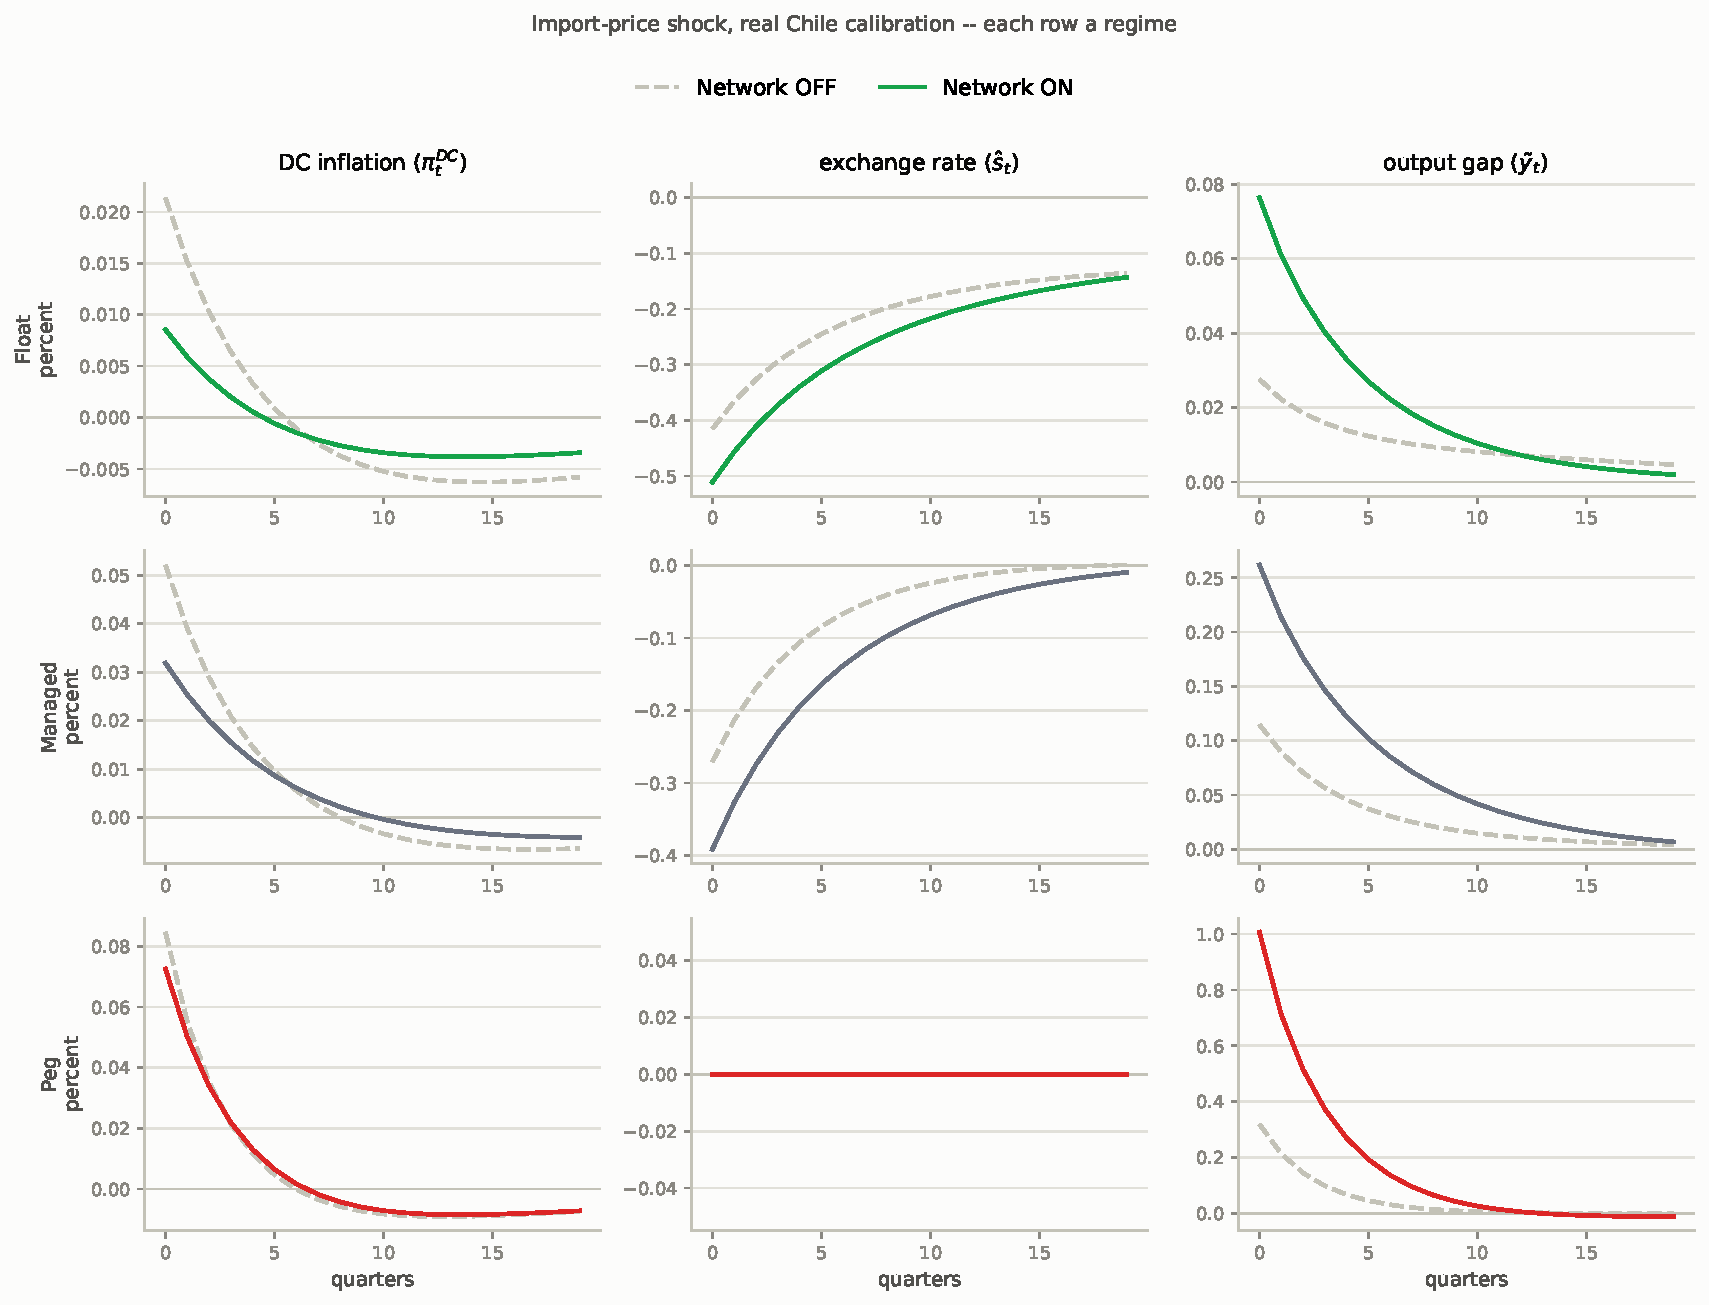
\includegraphics[width=0.62\textwidth]{figs/mechanism_network.pdf}
\end{center}

\end{frame}

%==============================================================
\begin{frame}{IRFs: Network ON vs.\ OFF --- Risk-Premium Shock}
%==============================================================

{\scriptsize Full IRFs behind the "Mechanism" slide's table: risk-premium/UIP shock, all three regimes, real Chile calibration --- \textbf{Network OFF} (dashed) vs.\ \textbf{Network ON} (solid):}

\begin{center}
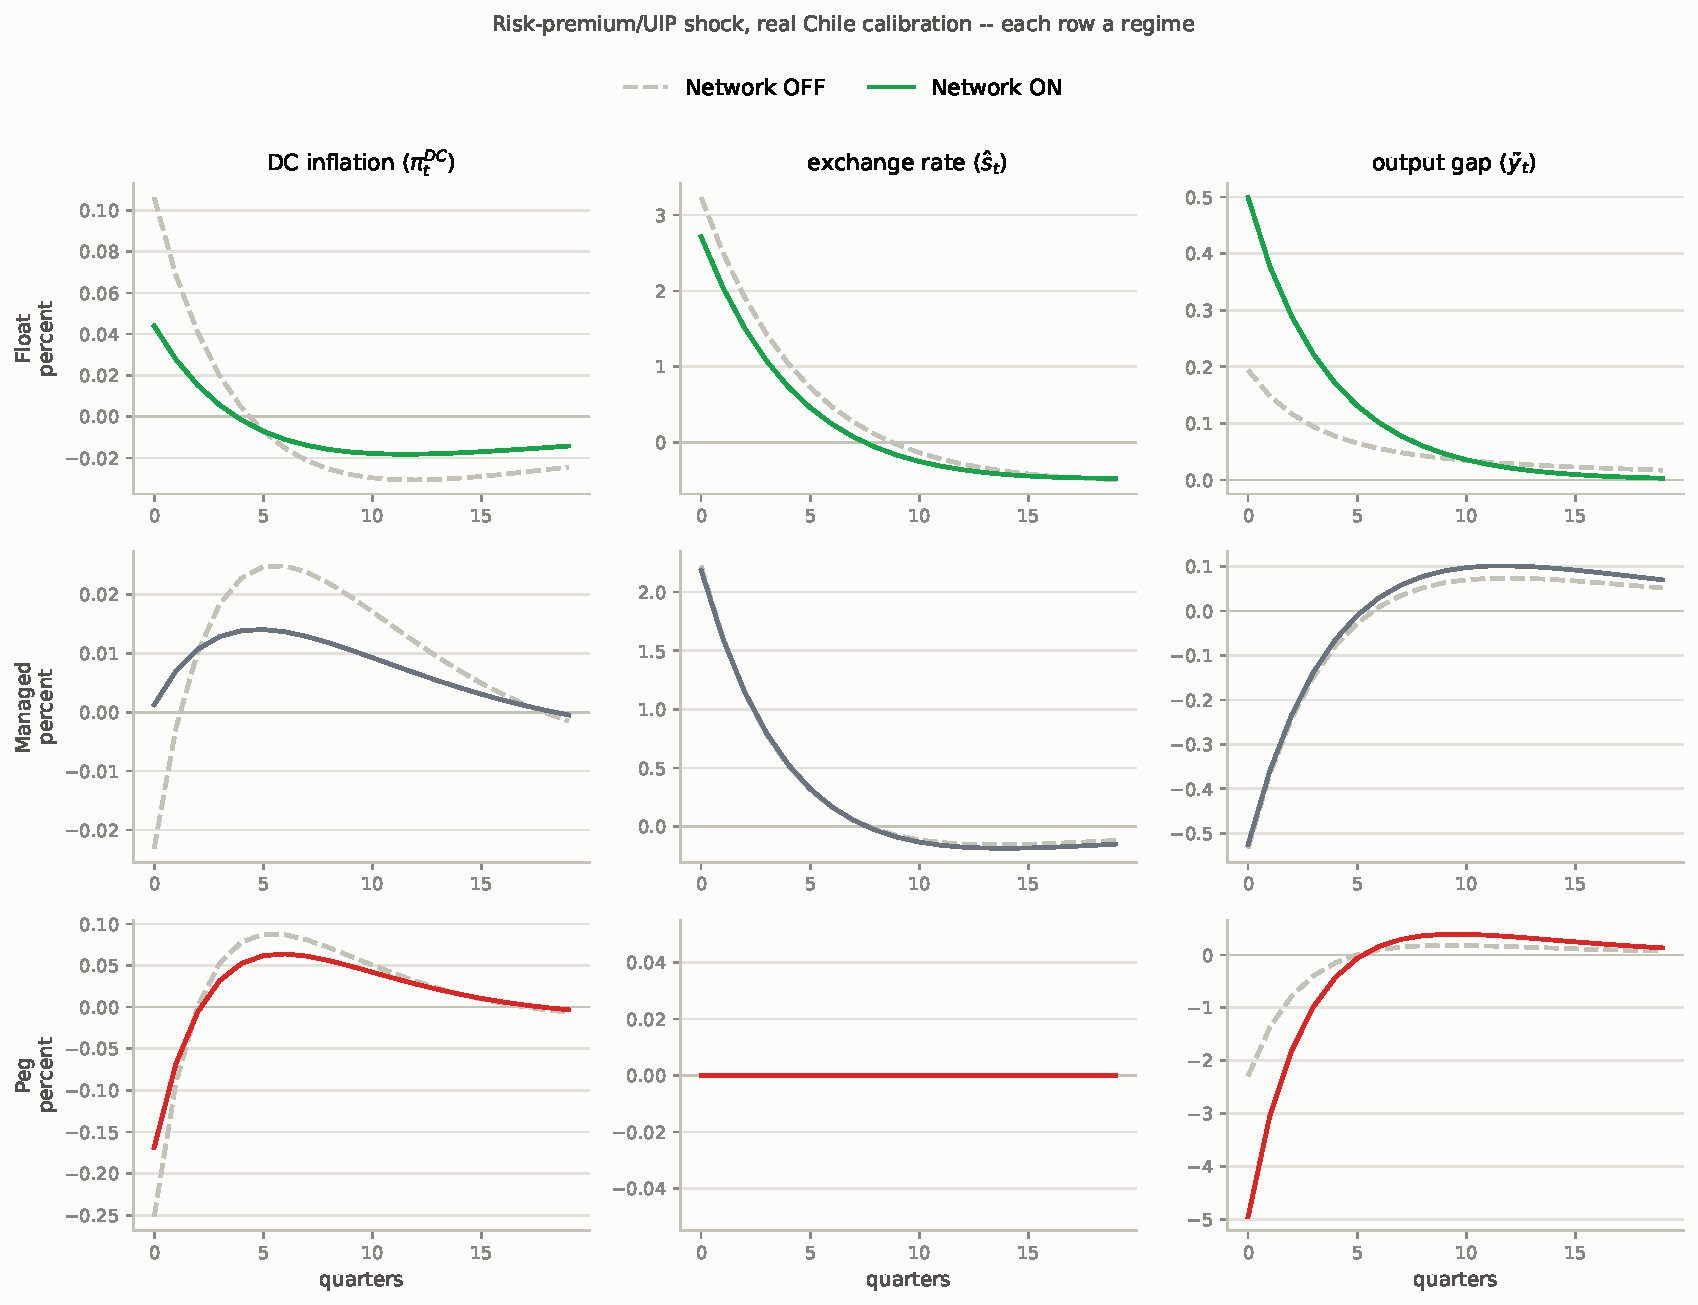
\includegraphics[width=0.62\textwidth]{figs/mechanism_network_rp.pdf}
\end{center}

\end{frame}

%==============================================================
\begin{frame}{Isolating the Network Channel: Sector Price-Dispersion Premium}
\hypertarget{netdenspremium}{}
%==============================================================

{\scriptsize Same density sweep as the main "Isolating the Network Channel" slide, but isolating only the \textbf{price-dispersion} piece of welfare ($\kappa_i\mathrm{Var}(\pi_{it})$), as a network premium $=$ value at $\rho{=}1$ minus value at $\rho{=}0$, by sector and regime:}

\vspace{4pt}
\begin{center}
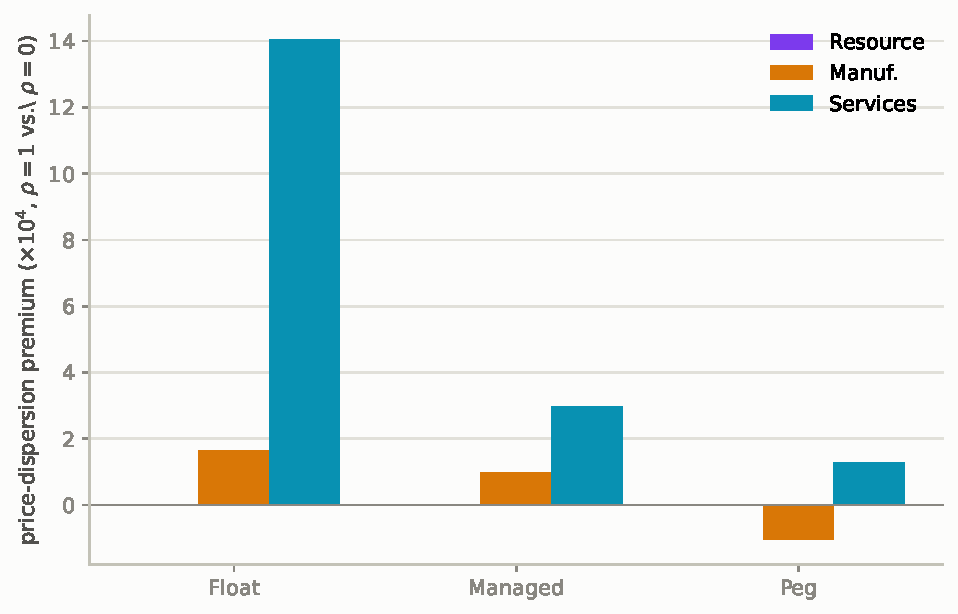
\includegraphics[width=0.62\textwidth]{figs/isolating_network_premium.pdf}
\end{center}

\vspace{4pt}
{\scriptsize
\begin{itemize}\setlength{\itemsep}{2pt}\setlength{\topsep}{0pt}
\item \textbf{Services is positive in every regime} (Float $3.39$, Managed $0.25$, Peg $0.37$) --- the network raises price-dispersion cost most where network centrality is highest ($\lambda_{D,\text{Services}}{=}1.11$)
\item \textbf{Manufacturing is negative in every regime}, most sharply under \textbf{Peg} ($-1.62$ vs.\ $-0.25$ Float, $-0.01$ Managed) --- Resource is near zero throughout
\item \textbf{Why Peg's price-dispersion premium doesn't dominate:} the network doesn't eliminate cost-push, it \textbf{redirects} it (see Mechanism slide) --- with no interest-rate room under a peg, most of the extra propagation shows up in the \textbf{output gap} instead (Peg's Services output-gap variance: $8.97\to35.16$, network OFF vs.\ ON, Network Exposure slide), not in this price-dispersion panel
\end{itemize}}

\end{frame}

%==============================================================
\begin{frame}{Robustness Summary: What Drives the Ranking?}
\hypertarget{robustsummary}{}
%==============================================================

\vspace{-6pt}
{\scriptsize \textbf{Managed $<$ Float $<$ Peg survives every sweep.} What changes is the \emph{size of the stakes} and \emph{who bears them}:}

\vspace{3pt}
{\tiny
\renewcommand{\arraystretch}{1.25}
\begin{tabular}{@{}p{2.2cm}p{4.9cm}p{2.4cm}@{}}
\toprule
\textbf{Dimension} & \textbf{Effect on the regimes} & \textbf{Ranking?} \\
\midrule
Import openness $\uparrow$ & Peg $\downarrow\downarrow$ (131$\to$68), Float $\uparrow$ (21$\to$44), Managed flat (11--13) & gap \textbf{converges} \\
Import concentration $\uparrow$ & Peg $\uparrow\uparrow$ (86$\to$93), Float/Managed roughly flat & gap \textbf{diverges} \\
Export openness $\uparrow$ & \textbf{all regimes improve}, Peg most (99$\to$85) & unchanged \\
Export concentration (Resource) & helps Peg, mildly hurts Float/Managed & unchanged \\
Network density $\rho\uparrow$ & \textbf{all} worsen, Peg fastest (73$\to$214 at $\rho{=}2.2$) & gap \textbf{diverges} \\
\bottomrule
\end{tabular}}

\vspace{3pt}
{\scriptsize
\begin{itemize}\setlength{\itemsep}{1.5pt}\setlength{\topsep}{0pt}
\item \textbf{Import side drives the ranking; export side barely does} --- consistent with the mechanism running through cost-push ($\Gamma\Delta e_t$), not terms-of-trade/expenditure-switching
\item \textbf{Volume vs.\ concentration point in opposite directions for Peg} --- more imports overall narrows the gap, but concentrating them in one sector widens it: it's exposure \emph{structure}, not import \emph{intensity}, that's dangerous
\item \textbf{Density is the one dimension where every regime worsens, but unevenly} --- Peg's loss grows fastest, so a more interconnected economy specifically strengthens the case against pegging
\item \textbf{A sector's own trade share is not what predicts its pain:} Services has the \emph{lowest} direct import share (7.0\%) but the \emph{largest} welfare cost --- it sits atop the Domar-weight chain ($\lambda_{D,\text{Services}}{=}1.11$) and inherits shocks from every sector upstream; network-off cuts its Peg output-gap cost by $75\%$ (35.16$\to$8.97)
\end{itemize}}

\end{frame}

%==============================================================
\section*{Appendix: Model Equations (Backup, not in 25-slide count)}
%==============================================================
\begin{frame}{Appendix: Model Equations \& Notation (1/2)}
\hypertarget{modeleqns}{}
%==============================================================

{\scriptsize\textbf{Households}}
\vspace{-2pt}
{\tiny
\[
\max\ \mathbb{E}_0\sum_t \beta^t\Big[\tfrac{C_t^{1-\gamma}}{1-\gamma} - \tfrac{L_t^{1+\varphi}}{1+\varphi}\Big]
\quad\text{s.t.}\quad
P^C_tC_t + S_tB^*_t = W_tL_t + \Pi_t + (1{+}i^*)\big[1{-}\psi(\hat b^*_{t-1}{-}\bar b^*)\big]S_tB^*_{t-1}
\]
\vspace{-8pt}
\[
C_t^{-\gamma} = \beta(1{+}i_t)\mathbb{E}_t\big[C_{t+1}^{-\gamma}/\Pi^C_{t+1}\big],\quad
W_t/P^C_t = C_t^{\gamma}L_t^{\varphi},\quad
(1{+}i_t) = (1{+}i^*)\big[1{-}\psi(\hat b^*_t{-}\bar b^*)\big]\,\mathbb{E}_t[S_{t+1}/S_t]\ \text{(UIP)}
\]}
{\tiny
\begin{tabular}{@{}llll@{}}
$C,L$: consumption, labor & $\beta,\gamma,\varphi$: discount, RRA, inv.\ Frisch & $W,i$: wage, dom.\ rate & $S,i^*$: ER, foreign rate \\
$\psi$: debt-elastic premium & $B^*$: foreign bond & $P^C$: CPI & $\Pi_t$: profits (rebated) \\
\end{tabular}}

\vspace{10pt}
{\scriptsize\textbf{Firms: Technology and Cost}}
\vspace{-2pt}
{\tiny
\[
Y_{it}=A_{it}\,L_{it}^{\alpha_i}\prod_j X_{ijt}^{\Omega^H_{ij}}\,M_{it}^{\Omega^F_i}
\quad\Rightarrow\quad
MC_{it}=\frac{W_t^{\alpha_i}\prod_j P_{jt}^{\Omega^H_{ij}}\,(S_tP^{F*}_t)^{\Omega^F_i}}{A_{it}}
\]
\vspace{-6pt}
\[
W_tL_{it}=\alpha_i MC_{it}Y_{it},\quad P_{jt}X_{ijt}=\Omega^H_{ij}MC_{it}Y_{it},\quad S_tP^{F*}_tM_{it}=\Omega^F_i MC_{it}Y_{it}
\]}
{\tiny
\begin{tabular}{@{}llll@{}}
$Y,A$: output, TFP & $L,X,M$: labor, dom./imp.\ inputs & $\Omega^H_{ij}$: dom.\ IO share & $\Omega^F_i$: import cost share \\
$\alpha_i$: labor share & $MC_{it}$: nominal marg.\ cost & \multicolumn{2}{l}{$P^{F*}$: foreign import price} \\
\end{tabular}}

\vspace{6pt}
{\footnotesize \textbf{Key:} $MC_{it}$ moves with both $A_{it}$ (TFP) and $S_t$ (via $M_{it}$) --- the two cost-push channels.}

\end{frame}

%==============================================================
\begin{frame}{Appendix: Model Equations \& Notation (2/2)}
%==============================================================

{\scriptsize \textbf{Firms: Calvo Pricing} --- reset price (probability $\delta_i$ resets, $1{-}\delta_i$ keeps last price):}
\vspace{-4pt}
{\tiny
\[
X1_{it} = \widetilde{MC}_{it}Y_{it} + (1{-}\delta_i)\beta\Big(\tfrac{C_{t+1}}{C_t}\Big)^{-\gamma}\Pi_{i,t+1}^{\varepsilon}X1_{i,t+1},\quad
X2_{it} = Y_{it} + (1{-}\delta_i)\beta\Big(\tfrac{C_{t+1}}{C_t}\Big)^{-\gamma}\Pi_{i,t+1}^{\varepsilon-1}X2_{i,t+1}
\]
\vspace{-8pt}
\[
P_{it}^\#/P_{it} = \tfrac{\varepsilon}{\varepsilon-1}\,X1_{it}/X2_{it},\quad
1 = (1{-}\delta_i)\Pi_{it}^{\varepsilon-1} + \delta_i \big(P_{it}^\#/P_{it}\big)^{1-\varepsilon},\quad
\hat\delta_i=\dfrac{\delta_i(1-\beta(1-\delta_i))}{1-\beta\delta_i(1-\delta_i)}
\]}
{\tiny
\begin{tabular}{@{}llll@{}}
$\delta_i$: Calvo reset prob.\ (primitive) & $\hat\delta_i$: derived slope (enters DC weights) & $P_{it}^\#$: reset price & $\varepsilon$: elasticity (markup $\varepsilon/(\varepsilon{-}1)$) \\
\end{tabular}}

\vspace{10pt}
{\scriptsize\textbf{Open Economy}}
\vspace{-2pt}
{\tiny
\[
\underbrace{P^{FH}_t = S_t P^{F*}_t}_{\text{LOP}},\quad
\underbrace{(1{+}i_t) = (1{+}i^*)\big[1{-}\psi(\hat b^*_t{-}\bar b^*)\big]\,\mathbb{E}_t[S_{t+1}/S_t]}_{\text{UIP}}
\]
\vspace{-8pt}
\[
\hat b^*_t = \tfrac{1+i_{t-1}}{\Pi^C_t}\hat b^*_{t-1} + \tfrac{P^H_t\sum_iEX_{it} - P^{FH}_t IM_t}{P^C_t},\quad
EX_{it} = \kappa_{EX,i}D^*_t\Big(\tfrac{P_{it}}{P^{FH}_t}\Big)^{-\theta^*}
\]
\vspace{-8pt}
\[
Y_{it} = \beta^H_i\tfrac{P^H_t}{P_{it}}C^H_t + \tfrac{P^H_t}{P_{it}}EX_{it} + \sum_j \Omega^H_{ji}\tfrac{MC_{jt}Y_{jt}}{P_{it}}
\]}
{\tiny
\begin{tabular}{@{}llll@{}}
$\hat b^*$: NFA (scaled) & $EX_i,IM$: sector exports, imports & $\theta^*$: export elasticity & $D^*$: foreign demand shifter \\
$\beta^H_i$: cons.\ share, sector $i$ & $\kappa_{EX,i}$: export-demand scale (baseline: sector-specific) & \multicolumn{2}{l}{Float: $i_t$ Taylor rule, $S_t$ free \quad Peg: $S_t=\bar S$, $i_t$ residual} \\
\end{tabular}}

\end{frame}

%==============================================================
\section*{Appendix: Extended Literature Review (Backup)}
%==============================================================
\begin{frame}{Appendix: The Peg vs.\ Float Debate --- What Do We Know?}
\hypertarget{littfull}{}
%==============================================================

{\footnotesize \textbf{Why it depends} (structure):}
{\scriptsize
\begin{itemize}\setlength{\itemsep}{1pt}
\item \textbf{Mundell (1961)} OCA --- fix favored by small, open, factor-mobile economies w/ correlated shocks vs.\ anchor; float favored by large, diversified ones
\item \textbf{Frankel (1999)} --- ``no single regime is right for all countries or at all times''; openness, size, trade \& capital-market structure all matter
\end{itemize}}

\vspace{2pt}
{\footnotesize \textbf{Shock-absorption view} (why float wins on real shocks --- robustly):}
{\scriptsize
\begin{itemize}\setlength{\itemsep}{1pt}
\item \textbf{Friedman (1953)} --- $S_t$ adjusts instead of costly wage/price deflation
\item \textbf{Broda (2004)} --- 75 dev.\ countries, 1973--96: negative ToT shocks $\to$ large real GDP declines under pegs
\item \textbf{Edwards \& Levy-Yeyati (2005)} --- 10\% ToT deterioration: $-0.80$pp growth under pegs vs.\ $-0.43$pp under floats
\item \textbf{Céspedes, Chang \& Velasco (2004)} --- even with dollarized-liability balance-sheet effects, float \emph{still} beats fixed
\end{itemize}}

\vspace{2pt}
{\footnotesize \textbf{But floating is not a free lunch} (limits on float's insulation):}
{\scriptsize
\begin{itemize}\setlength{\itemsep}{1pt}
\item \textbf{Calvo \& Reinhart (2002)} ``Fear of Floating'' --- EMEs peg de facto anyway: credibility-building, not literal welfare optimum
\item \textbf{Rey (2013)} ``Dilemma not trilemma'' --- under free capital mobility, float alone doesn't deliver monetary autonomy
\end{itemize}}

\vspace{3pt}
{\scriptsize \textbf{Consensus:} no corner solution is universally optimal --- the choice trades a nominal anchor against real-shock absorption, shock- and structure-dependent.}

\end{frame}

%==============================================================
\begin{frame}{Appendix: The Frontier --- Is Fear of Floating Actually Optimal?}
%==============================================================

{\scriptsize
\begin{itemize}\setlength{\itemsep}{5pt}
\item \textbf{Itskhoki \& Mukhin (2023)} --- general open-economy framework with endogenous UIP/PPP deviations: efficient policy $=$ MP closes the output gap $+$ FX intervention eliminates the UIP wedge. Optimal policy is generically a \textbf{managed float/crawling peg}, matching observed fear of floating. When the natural RER is stable, this collapses to an ``open-economy divine coincidence.''
\\ \textcolor{customgreen!55!black}{$\hookrightarrow$ \emph{vs.\ us:}} \textbf{same headline} (Managed, not a corner, is optimal) --- reached instead via a multi-sector Calvo network with a persistence-driven, not UIP-gap-closing, mechanism

\item \textbf{Bianchi \& Coulibaly (2025; 2022 WP)} --- fear of floating is \textbf{optimal}, not behavioral, when credit access is tied to the real exchange rate (self-fulfilling crisis risk). Prescription: float for real shocks, \textbf{fix} for financial shocks
\\ \textcolor{customgreen!55!black}{$\hookrightarrow$ \emph{vs.\ us:}} \textbf{opposite ranking} for our financial shock --- our risk-premium/UIP shock passes straight through under \textbf{Peg} (worst regime). Different financial friction (persistent NFA wedge vs.\ collateral-constraint crisis) flips the prescription

\item \textbf{Coulibaly (2023)} --- discretionary MP is procyclical to offset balance-sheet effects; commitment (inflation targeting) or capital controls raise welfare
\\ \textcolor{customgreen!55!black}{$\hookrightarrow$ \emph{vs.\ us:}} echoes our ``Managed $=$ extra instrument'' logic --- giving policy more tools beats a corner regime
\end{itemize}}

\vspace{4pt}
{\scriptsize \textbf{Bottom line:} the 2023--25 frontier has also moved past corner solutions --- but \emph{why} fear of floating is optimal is mechanism-specific. We add production-network amplification $+$ shock persistence as a distinct reason, not examined by either paper.}

\end{frame}

%==============================================================
\begin{frame}{Appendix: How Our Results Compare to the Literature}
%==============================================================

{\tiny
\renewcommand{\arraystretch}{1.05}
\begin{tabular}{@{}p{2.8cm}p{3.55cm}p{3.55cm}@{}}
\toprule
\textbf{Literature} & \textbf{Says} & \textbf{Us} \\
\midrule
Mundell (1961); Frankel (1999) & Optimal regime depends on structure, no universal answer & \textbf{Confirms}: ranking flips with shock type (UIP vs.\ TFP) and network density \\[1pt]
Friedman (1953); Broda (2004); Edwards--Levy-Yeyati (2005); Céspedes--Chang--Velasco (2004) & Float buffers real (ToT/foreign) shocks, lower output loss than peg --- robust even to balance-sheet effects & \textbf{Same direction} (Peg worst), \textbf{different shock}: risk-premium/UIP, not ToT \\[1pt]
Gal\'i \& Monacelli (2005) & Peg dominated, float $\approx$ optimal in 1-sector SOE & \textbf{Same ranking of Peg}, but pure \textbf{Float is not optimal}: Managed beats it \\[1pt]
Calvo--Reinhart (2002) & EMEs avoid pure float --- read as \textbf{fear}, a credibility-driven deviation from optimum & We find partial stabilization is \textbf{literally welfare-optimal} --- a persistence-driven, not fear-driven, reason \\[1pt]
Rey (2013) & Float alone doesn't insulate; need a second instrument (capital controls/macropru) & Echoes Fanelli--Straub: Managed uses $S_t$ itself as that \textbf{second instrument} \\[1pt]
Qiu, Wang, Xu \& Zanetti (2026, JME) & Open-economy DC index (CPI+expenditure-switching+profit channels), \emph{static}, WIOD-calibrated; DC breaks down, output-gap targeting near-optimal & \textbf{Independent corroboration} DC breaks down in open economy; \textbf{we add} the piece they flag as their own top open extension --- UIP, NFA persistence, and FX-\textbf{regime choice} \\
\bottomrule
\end{tabular}}

\vspace{4pt}
{\scriptsize \textbf{Novel angle:} the classic shock-absorber logic (Friedman/Broda) is about shock \textbf{type} (real vs.\ nominal). Our driver is a shock \textbf{property} --- persistence (near-unit-root NFA) --- not previously emphasized in this literature.}

\end{frame}

%==============================================================
\section*{Appendix: ECB Open-Economy Production-Network Model (Backup)}
%==============================================================
\begin{frame}{Appendix: The ECB's Open-Economy Production-Network Model}
\hypertarget{ecbnetwork}{}
%==============================================================

{\scriptsize \textbf{Gnocato, Montes-Gald\'on \& Stamato (2025)}, ``Tariffs across the supply chain,'' ECB WP No.\ 3081 --- also underlies Lane's (ECB Exec.\ Board) 13 May 2026 speech on energy shocks (4-region extension):}
{\scriptsize
\begin{itemize}\setlength{\itemsep}{1pt}\setlength{\topsep}{2pt}
\item \textbf{Setup:} two-region, multi-sector, full IO structure, international production network; sticky wages/prices; Taylor rule on \emph{domestic} CPI (no regime comparison)
\item \textbf{Finding:} tariffs on \textbf{intermediate} inputs $\to$ persistent inflation \& larger GDP loss; tariffs on \textbf{final} goods $\to$ one-off spike, smaller loss --- \emph{where} in the network a shock hits sets its persistence
\item \textcolor{customgreen!55!black}{$\hookrightarrow$ \emph{vs.\ us:}} their tariff-location result and our TFP-vs-UIP result are the same insight: shock \textbf{location/type} sets its persistence
\end{itemize}}

\vspace{2pt}
{\scriptsize \textbf{What it cites for open economy $+$ production networks:}}
{\tiny
\begin{itemize}\setlength{\itemsep}{1pt}\setlength{\topsep}{2pt}
\item Network amplification, closed economy: \textbf{Pasten, Schoenle \& Weber (2020)}; \textbf{Ghassibe (2021)}; \textbf{Rubbo (2023)}\footnote{\tiny Published as Rubbo, E. (2023), Econometrica 91(4), 1417--1455.}; \textbf{Afrouzi \& Bhattarai (2023)}
\item Open-economy multi-sector NK $+$ networks: \textbf{Devereux, Gente \& Yu (2023)}; \textbf{Hinterlang et al.\ (2023)} EMuSe (Bundesbank); closest: \textbf{Kalemli-\"Ozcan, Soylu \& Yildirim (2025)} ``Global networks, MP and trade''
\item Trade fragmentation \& inflation: \textbf{Moro \& Nispi Landi (2024)}; \textbf{Ambrosino, Chan \& Tenreyro (2026, \emph{JIE})}
\item Optimal MP under tariffs: \textbf{Bergin \& Corsetti (2023)}; \textbf{Bianchi \& Coulibaly (2025)} ``Optimal MP response to tariffs'' (\emph{different} paper from their fear-of-floating one)
\end{itemize}}

\vspace{2pt}
{\scriptsize \textbf{Bottom line:} none compares FX \textbf{regimes} or asks whether a DC index survives --- they fix the monetary rule.}

\end{frame}

